% Options for packages loaded elsewhere
\PassOptionsToPackage{unicode}{hyperref}
\PassOptionsToPackage{hyphens}{url}
\PassOptionsToPackage{dvipsnames,svgnames,x11names}{xcolor}
\documentclass[
  11pt,
  letterpaper,
]{article}
\usepackage{xcolor}
\usepackage[margin=1in]{geometry}
\usepackage{amsmath,amssymb}
\setcounter{secnumdepth}{-\maxdimen} % remove section numbering
\usepackage{iftex}
\ifPDFTeX
  \usepackage[T1]{fontenc}
  \usepackage[utf8]{inputenc}
  \usepackage{textcomp} % provide euro and other symbols
\else % if luatex or xetex
  \usepackage{unicode-math} % this also loads fontspec
  \defaultfontfeatures{Scale=MatchLowercase}
  \defaultfontfeatures[\rmfamily]{Ligatures=TeX,Scale=1}
\fi
\usepackage{lmodern}
\ifPDFTeX\else
  % xetex/luatex font selection
  \setmainfont[]{Arial}
\fi
% Use upquote if available, for straight quotes in verbatim environments
\IfFileExists{upquote.sty}{\usepackage{upquote}}{}
\IfFileExists{microtype.sty}{% use microtype if available
  \usepackage[]{microtype}
  \UseMicrotypeSet[protrusion]{basicmath} % disable protrusion for tt fonts
}{}
\makeatletter
\@ifundefined{KOMAClassName}{% if non-KOMA class
  \IfFileExists{parskip.sty}{%
    \usepackage{parskip}
  }{% else
    \setlength{\parindent}{0pt}
    \setlength{\parskip}{6pt plus 2pt minus 1pt}}
}{% if KOMA class
  \KOMAoptions{parskip=half}}
\makeatother
\usepackage{longtable,booktabs,array}
\newcounter{none} % for unnumbered tables
\usepackage{calc} % for calculating minipage widths
% Correct order of tables after \paragraph or \subparagraph
\usepackage{etoolbox}
\makeatletter
\patchcmd\longtable{\par}{\if@noskipsec\mbox{}\fi\par}{}{}
\makeatother
% Allow footnotes in longtable head/foot
\IfFileExists{footnotehyper.sty}{\usepackage{footnotehyper}}{\usepackage{footnote}}
\makesavenoteenv{longtable}
\usepackage{graphicx}
\makeatletter
\newsavebox\pandoc@box
\newcommand*\pandocbounded[1]{% scales image to fit in text height/width
  \sbox\pandoc@box{#1}%
  \Gscale@div\@tempa{\textheight}{\dimexpr\ht\pandoc@box+\dp\pandoc@box\relax}%
  \Gscale@div\@tempb{\linewidth}{\wd\pandoc@box}%
  \ifdim\@tempb\p@<\@tempa\p@\let\@tempa\@tempb\fi% select the smaller of both
  \ifdim\@tempa\p@<\p@\scalebox{\@tempa}{\usebox\pandoc@box}%
  \else\usebox{\pandoc@box}%
  \fi%
}
% Set default figure placement to htbp
\def\fps@figure{htbp}
\makeatother
\setlength{\emergencystretch}{3em} % prevent overfull lines
\providecommand{\tightlist}{%
  \setlength{\itemsep}{0pt}\setlength{\parskip}{0pt}}
\usepackage{bookmark}
\IfFileExists{xurl.sty}{\usepackage{xurl}}{} % add URL line breaks if available
\urlstyle{same}
\hypersetup{
  pdftitle={Open3DCP: A Public Data Schema for 3D Concrete Printing},
  pdfauthor={Nicholas Sonnentag --- Sunnyday Technologies, Wisconsin, USA},
  colorlinks=true,
  linkcolor={[HTML]{013A73}},
  filecolor={Maroon},
  citecolor={Blue},
  urlcolor={Blue},
  pdfcreator={LaTeX via pandoc}}

\title{Open3DCP: A Public Data Schema for 3D Concrete Printing}
\usepackage{etoolbox}
\makeatletter
\providecommand{\subtitle}[1]{% add subtitle to \maketitle
  \apptocmd{\@title}{\par {\large #1 \par}}{}{}
}
\makeatother
\subtitle{Design, rationale, and the measurement gaps of an
analysis-ready record for extrusion 3D concrete printing}
\author{Nicholas Sonnentag --- Sunnyday Technologies, Wisconsin, USA}
\date{2026-07-30}

\begin{document}
\maketitle

{
\setcounter{tocdepth}{2}
\tableofcontents
}
\section{Abstract}\label{abstract}

Three-dimensional concrete printing (3DCP) is a coupled
material--process problem: a printable cementitious system is defined by
composition, rheology, equipment, toolpath, environmental exposure,
curing, specimen extraction, test orientation, and measured performance.
The literature reports many of these facts, but distributes them across
prose, tables, figures, and supplementary files using inconsistent names
and unit bases --- which makes cross-study comparison, meta-analysis,
and machine-learning workflows harder than the underlying measurements
require. Open3DCP is an open, flat schema for recording extrusion-based
3DCP mix-design and test records. Version 1.7.5 defines \textbf{248
columns} in its primary record, spanning composition, fibers,
admixtures, fresh-state rheology, 3DCP process parameters, hardened
mechanical and durability properties, interlayer bond, specimen/test
metadata, environmental conditions, and provenance. Quantities are
recorded on a \textbf{dual basis that keeps kg/m³ --- the field standard
--- first-class}: the constituent columns store the self-normalizing
mass-percent projection, and bridge columns preserve the source's kg/m³
exactly, so either basis is recoverable without a density assumption;
missingness is represented as \texttt{NULL}, with \texttt{0} reserved
for explicit source-reported zero. Open3DCP is a \emph{reporting layer},
not a test method or a substitute for ASTM, EN, ACI, ICC, ISO, or RILEM
standards: it lets 3DCP records be assembled into interoperable datasets
for scientific review, Integrated Computational Materials Engineering
(ICME)--style process--structure--property analysis, digital-twin
reconstruction, and downstream analysis where sufficient validated data
exist. We give the design rationale for each major decision and
\textbf{demonstrate ingestion} on five openly-licensed public datasets
--- a cast-concrete benchmark, a corporate carbon-aware set, a
\textasciitilde30-laboratory 3DCP mechanical database, an extrusion-3DCP
printability set, and a project-layer building catalogue --- into one
schema, including a cross-study print-anisotropy result. The point
Open3DCP makes is one of \textbf{characterization, not prediction}: each
source records a different slice of the material and process ---
composition, fresh-state rheology, hardened performance, embodied
carbon, print orientation, or the as-built project --- and the schema
holds their union in one shape, so that what any one study leaves
unmeasured is made explicit rather than lost. We also identify a
taxonomy of features that are physically important but cannot yet be
measured reliably --- an agenda for instrumentation.

\section{Contributions}\label{contributions}

\begin{itemize}
\tightlist
\item
  An open, \textbf{3DCP-native flat data schema} (v1.7.5, 248 columns)
  with first-class columns for print process parameters, fresh-state
  rheology, and interlayer-bond properties --- the features that
  distinguish printed concrete from cast.
\item
  A \textbf{design rationale} for each consequential choice: flat table
  over graph, \emph{dual-basis} recording that keeps kg/m³ first-class,
  fineness-modulus over maximum aggregate size, and \texttt{NULL} ≠
  \texttt{0}.
\item
  A \textbf{measurement-gap taxonomy} --- real-time process monitoring,
  in-situ material state, and post-process characterization gaps ---
  framed as a research agenda for instrumentation.
\item
  A \textbf{worked demonstration} ingesting five openly-licensed public
  datasets --- a cast-concrete benchmark, a corporate carbon-aware set,
  a \textasciitilde30-laboratory 3DCP mechanical database, an
  extrusion-3DCP printability set, and a project-layer building
  catalogue --- into one schema, two of them carrying a real automated
  fidelity score, and yielding a cross-study print-anisotropy result
  that the schema's orientation field makes expressible (§6).
\end{itemize}

\begin{center}\rule{0.5\linewidth}{0.5pt}\end{center}

\subsection{1. Introduction}\label{introduction}

3D concrete printing has moved from laboratory demonstrations toward
construction-scale experimentation; printed residential structures,
bridges, and architectural elements have been produced in many countries
worldwide using systems ranging from gantry extruders to six-axis
robotic arms {[}1, 2, 3{]}. The technical literature now spans printable
mortars, alkali-activated binders, fiber-reinforced systems, recycled
aggregates, interlayer bond, anisotropic strength, rheology,
buildability, and durability. The public record is large enough to
support comparative analysis, but not yet consistently shaped enough to
make that analysis straightforward.

The central problem is not that researchers fail to report data --- many
papers report substantial detail --- but that the detail is not
represented in a common structure. A material may appear as ``GGBFS,''
``slag,'' ``ground granulated blast-furnace slag,'' or a supplier name;
a dosage may be reported in kg/m³, percent of binder, or percent of
total mass; a compressive strength may refer to a cast cube, a printed
prism, a cored specimen, or a coupon loaded across the layer interface.
These distinctions matter scientifically, yet they are often not
preserved in a machine-readable way. The consequence is direct: datasets
from different groups cannot be combined without extensive manual
harmonization, so the field cannot easily build the large, multi-source
corpora that modern analysis needs. The most widely used concrete
dataset for machine learning --- Yeh's UCI Concrete Compressive Strength
set {[}4{]} --- captures only composition and age, with no process,
rheology, or orientation fields, and predates 3DCP entirely (§3).

What makes 3DCP fundamentally different from cast concrete can be stated
in four points:

\begin{enumerate}
\def\labelenumi{\arabic{enumi}.}
\tightlist
\item
  \textbf{Process--property coupling.} The same mix, printed at
  different speeds, layer heights, and time gaps, can produce
  substantially different mechanical properties. Process parameters are
  design variables, not noise.
\item
  \textbf{Anisotropy.} Printed concrete is direction-dependent;
  specimens tested across the layer interface can be 20--40 \% weaker
  than those tested parallel to the layers {[}5, 6{]}. A strength value
  without an orientation is ambiguous.
\item
  \textbf{Rheological demands.} The mix must be simultaneously pumpable
  and buildable; yield stress, thixotropy, and open time are critical
  performance parameters absent from conventional concrete datasets
  {[}7{]}.
\item
  \textbf{Interlayer bond.} The weakest link in a printed element is
  usually the interface between layers, where bond depends on surface
  moisture, time gap, ambient conditions, and degree of hydration at
  deposition {[}8, 9{]}.
\end{enumerate}

These four properties are what a 3DCP record has to capture if
printed-concrete results are to be compared across studies at all: a
strength without a process, a rheology, and an orientation is not a
comparable measurement. Open3DCP exists to record that fuller
experiment, not to model it.

\subsection{2. Scope and non-scope}\label{scope-and-non-scope}

Open3DCP is a schema specification: it defines \emph{how} to record
data; it does not provide the data. It is scoped to
\textbf{extrusion-based (material-extrusion / FDM-style) 3D concrete
printing} --- the process whose pump, nozzle, layer schedule, and
toolpath the schema captures. Particle-bed / binder-jetting, spray, and
slip-form methods are out of scope: they have different process
variables and would need their own process block.

On materials chemistry, Open3DCP covers \textbf{hydraulic cementitious
systems} --- Portland and blended cements, calcium-aluminate and
calcium-sulfoaluminate cements, and high-calcium alkali-activated slag,
whose C-(A-)S-H binding gel is chemically continuous with Portland
hydrates. Low-calcium fly-ash \textbf{geopolymers} (whose N-A-S-H gel is
a distinct binder chemistry) are out of scope; the schema's activator
columns exist to record the high-calcium alkali-activated systems that
are in scope, not to characterize geopolymers.

Open3DCP \textbf{is}:

\begin{itemize}
\tightlist
\item
  A public column vocabulary for 3DCP mix-design and test records.
\item
  A dual-basis, SI-unit reporting convention: mass-percent stored, the
  source's kg/m³ (the field standard) preserved exactly via bridge
  columns --- either basis recoverable without assumption.
\item
  A standards-aligned cross-reference layer for common material classes
  and test methods.
\item
  A flat structure for CSV, SQL, Parquet, dataframe, and
  repository-deposit workflows.
\item
  A citable artifact with a DOI and Apache-2.0 licensing.
\end{itemize}

Open3DCP \textbf{is not}:

\begin{itemize}
\tightlist
\item
  A dataset or benchmark, a database service, or an API.
\item
  A structural-design method or a code-compliance path.
\item
  A replacement for ASTM, EN, ACI, ICC, RILEM, ISO, or
  jurisdiction-specific requirements.
\item
  Evidence that any particular mix is safe, durable, printable, or
  construction-ready.
\end{itemize}

The schema can record data used in qualification or research workflows,
but any construction use still requires appropriate laboratory
validation, professional engineering review, and approval under the
governing jurisdiction.

\subsection{3. Background and related
work}\label{background-and-related-work}

\textbf{The ICME paradigm and lessons from metals additive
manufacturing.} The idea that materials can be designed from performance
requirements backward through processing--structure--property
relationships was advanced by Olson's work on hierarchical,
systems-based materials design {[}15, 16{]}; this approach was later
formalized as Integrated Computational Materials Engineering (ICME). The
Materials Genome Initiative {[}17{]} sought to extend it through data
infrastructure, funding repositories, ontologies, and schema patterns.
In parallel, the FAIR principles for scientific data --- Findable,
Accessible, Interoperable, Reusable --- were articulated by Wilkinson et
al.~{[}18{]}; together they shaped the data-stewardship practices
Open3DCP follows. Metals additive manufacturing offers a particularly
instructive parallel: early laser-powder-bed and
directed-energy-deposition work used ad-hoc formats until ASTM F3049
{[}10{]} and the NIST AM Bench program established common reporting
practices that enabled cross-laboratory comparison. That effort took
most of a decade; 3DCP is at the start of a similar trajectory. The key
insight carried over is that \textbf{the manufacturing process is a
design variable, not a constraint} --- printable concrete should be
purpose-designed for layer-by-layer deposition, and capturing that
requires a record of what makes extrusion different from casting.

\textbf{Seminal work in 3D concrete printing.} Automated construction
with cementitious materials dates to Pegna's solid-freeform work
{[}19{]}; Khoshnevis developed Contour Crafting {[}20{]} and Cesaretti
et al. demonstrated binder-jetting of regolith simulant {[}21{]}. The
modern extrusion era began with two groups in parallel: at Loughborough,
Buswell, Lim, Le and colleagues published early mix-design and
construction-scale studies {[}22, 23{]}; at TU Eindhoven, Bos, Wolfs,
Ahmed and Salet produced early structural printed elements --- including
a 3D-printed concrete bridge designed by testing {[}1, 24{]} --- with
Wolfs et al.~on early-age behaviour {[}5{]} and Suiker on wall stability
{[}25{]}. Roussel established the rheological framework for printable
concrete {[}7{]}, and Perrot et al.~quantified structural build-up
{[}26{]}. The NTU Singapore group contributed systematic rheology
studies including geopolymers {[}27, 28{]}, printability regions
{[}29{]}, and fresh/hardened characterization {[}30{]}. Interlayer bond
--- the defining weakness --- has been studied by Kruger, van Zijl and
colleagues on porosity {[}6{]}, Sanjayan et al.~on surface moisture
{[}8{]}, Moelich et al.~on quantitative bond models {[}9{]}, Van Der
Putten et al.~on surface modification {[}31{]}, and Marchment and
Sanjayan on mesh reinforcement {[}32{]}. Structural implications were
addressed by Asprone et al.~{[}33{]} and Gebhard et al.~{[}34{]}.
Broader reviews include Mechtcherine et al.~on production physics
{[}35{]}, Buswell et al.'s research roadmap {[}3{]}, Nerella et al.~on
strain-based build-up {[}36{]}, De Schutter et al.~on
technical/economic/environmental potentials {[}2{]}, large-scale UHPC
work {[}37{]}, a classification of building systems {[}38{]},
particle-bed printing {[}39{]}, fiber-reinforced and recycled-aggregate
formulations {[}40, 41{]}, the 3DCP.fyi citation network {[}42{]}, and
Wangler et al.'s digital-concrete review {[}43{]}; the RILEM TC 276-DFC
state-of-the-art report consolidates digital-fabrication practice
{[}46{]}.

\textbf{Standards development.} RILEM TC 304-ADC has driven test-method
standardization for 3DCP; its interlaboratory study coordinated testing
across roughly thirty laboratories and quantified inter-laboratory
variability {[}11, 12, 13{]}, with an accompanying database system for
sharing experimental data {[}14{]}. Vasilić reviewed the state of
standardization, identifying the gap between established \emph{test
methods} (which RILEM provides) and a unified \emph{data schema} for
analysis-ready storage (which no formal standard yet provides) {[}44{]}.
Conventional standards --- ACI 318 for structural design, ASTM C39
(compressive), C496 (splitting tensile), C1583 (pull-off direct
tension), C78 (flexural), C469 (modulus), C191 (setting), C1611 (slump
flow), and the EN 197/206/12390 series --- supply the measurement
framework 3DCP inherits, but were written for cast concrete; the test
methods remain valid while the \emph{conditions} of production and the
\emph{metadata} needed to interpret results differ.

\textbf{Semantic data models and ontologies.} Between test-method
standards and datasets sits a further body of precedent: general-purpose
data models and ontologies for manufacturing and materials data. In
additive manufacturing broadly, a joint industry--government working
group produced the AM Common Data Dictionary, whose process-agnostic
core is standardized as ASTM F3490-21 {[}53{]}, and the open-source AM
Common Data Model (AM-CDM) {[}52{]}. AM-CDM's six modules (base,
material, system, process, build, and
test--inspection--characterization) define a relationship-first exchange
structure that organizations are expected to \emph{map to} rather than
adopt as storage; its material module is currently metals-shaped, and no
cementitious or construction profile exists. In materials science, the
Platform MaterialDigital core ontology (PMDco) provides a mid-level
process--structure--property scaffold {[}54{]}; Citrine's GEMD format
expresses materials histories as linked spec/run objects {[}59{]}; and
PMDco's concrete-domain extension --- the LeBeDigital Concrete
Production and Testing Ontology (CPTO) --- models the EN 206
cast-concrete production chain, from constituents and mix quantities
through fresh and hardened testing and conformity, yet contains no
printing, extrusion, structural-build-up, or interlayer concepts
{[}55{]}. In construction informatics, the Building Concrete Monitoring
Ontology (BCOM) covers the cast-in-place QA chain (delivery, placement,
curing, specimens, strength conformity) for BIM-linked asset management
{[}56{]}. Additive construction itself is an active ontology-research
direction: the TRR 277 ontology suite of Li and Petzold spans concrete
composition, printing systems, and building design under BFO/IOF (Basic
Formal Ontology / Industrial Ontologies Foundry) top-level alignment
{[}57{]}, and the Printing Information Modeling ontology of Peralta
Abadia et al.~links mix design, material--process interaction, and
toolpath data to BIM {[}58{]}; neither has yet released a public
ontology artifact.

Open3DCP does not compete with these frameworks. They are
relationship-first exchange and reasoning layers; Open3DCP is the flat,
analysis-ready record a 3DCP experiment is \emph{reported in} --- in
effect a candidate for the 3DCP domain profile those general models
currently lack. Its composition, condition, and property blocks map onto
AM-CDM's material and test modules, GEMD's spec/run objects, and CPTO's
constituent and test classes, while its printing-process, printing-state
rheology, and interlayer blocks are precisely the vocabulary none of
these precedents yet holds. An initial machine-readable crosswalk with
field-level mapping classes is included in the schema repository
(\texttt{crosswalk/}); calibrating and extending it is planned work
(§11).

\textbf{Existing datasets and their limitations.} The most cited ML
concrete dataset, Yeh's UCI set {[}4{]}, captures only composition and
age in kg/m³ (requiring a density assumption for formulation-level
comparison) and no process, rheology, orientation, specimen, or
provenance fields. Repositories such as Mendeley Data and Zenodo host
specialized concrete datasets, but --- to our knowledge --- none provide
a general-purpose 3DCP-native schema with first-class process
parameters. The closest prior art is the RILEM TC 304-ADC
interlaboratory database system {[}14{]}, the first multi-laboratory
3DCP dataset with standardized protocols; its schema, however, is scoped
to that interlaboratory study (its entity model covers materials,
specimens, and tests but not a general printing-process vocabulary),
whereas Open3DCP aims at a reusable, analysis-ready record across
studies. We position Open3DCP as complementary to {[}14{]}, not a
replacement.

\subsection{4. Why 3DCP needs a 3DCP-native
record}\label{why-3dcp-needs-a-3dcp-native-record}

Conventional concrete datasets focus on composition, age, and one or
more hardened properties --- useful for cast concrete, where placement
and compaction are treated as standardized. 3DCP makes that assumption
unsafe: the manufacturing process is part of the material definition. At
minimum, a 3DCP record must distinguish what was weighed into the mix;
how it was prepared and modified over time; how it was pumped and
extruded; what geometry was deposited; how much time elapsed between
adjacent layers; the environmental conditions during deposition; how the
specimen was cured and extracted; the loading direction relative to the
layer interface; the test method or local protocol; and whether each
value was measured, calculated, estimated, or merely reported. Without
these attributes, two identical-looking compressive strengths may
describe physically different experiments --- a cast cube and a printed
coupon loaded across interlayers should not collapse into one data point
merely because both report MPa.

\subsection{5. Schema design principles}\label{schema-design-principles}

Open3DCP is governed by a small set of principles, each motivated by the
practical requirements of analysis and the lessons of data
standardization in adjacent fields.

\textbf{5.1 Flat schema.} Every stored feature is a named column in a
single table --- no JSON nesting, no graph structure, no join required
for basic analysis. This prioritizes adoption by the researchers,
curators, and ML practitioners who overwhelmingly work with tabular data
(pandas, CSV, SQL) over the representational elegance of graph models
such as GEMD {[}59{]}, which capture provenance chains and measurement
hierarchies but add friction for the common ``load a table and train a
model'' use case. A graph view can be constructed from the flat schema
for the structure it captures; conversely, the flat row deliberately
omits the full relational/provenance tree (§9), so flat→graph
reconstruction is faithful only for the subset the row holds --- the two
are complementary, not equivalent.

\textbf{5.2 Dual basis: mass-percent stored, kg/m³ preserved.} To be
precise about what sits where: the constituent columns \textbf{store
mass-percent of total wet mix} --- the self-normalizing projection (Σ ≈
100 \%) that pools cleanly across datasets --- while the source's
\textbf{kg/m³} (the convention the concrete industry and field actually
use) is \textbf{preserved exactly and is first-class}, never
approximated. Three columns make the two interconvertible without
assumption: \texttt{original\_basis} records what the source reported
(\texttt{kg\_m3} \textbar{} \texttt{mass\_pct} \textbar{}
\texttt{volume} \textbar{} \texttt{lb\_yd3}), and
\texttt{total\_batched\_mass\_kg\_m3} and \texttt{total\_binder\_kg\_m3}
carry the batched-mass and binder totals needed to convert exactly in
either direction. This resolves a real tension: kg/m³ is what
practitioners report and need, but normally requires a density
assumption for cross-dataset comparison when density is unreported;
mass-percent is self-normalizing and ideal for pooled analysis, but is
foreign to field practice. Storing the projection plus the lossless
bridge serves both without discarding information. (Schema versions ≤
v1.5 carried mass-percent only, with no recoverable kg/m³; v1.7 added
the bridge columns that make kg/m³ exact. Admixtures are recorded on a
\textbf{solids basis} where the source reports the solids fraction;
where it does not --- common in public datasets --- the as-delivered
mass is stored \emph{exactly} and the row's \texttt{admixture\_basis}
flag records \texttt{as\_delivered} (v1.7.5), so nothing is assumed and
solids remain derivable when a fraction is known. \texttt{w\_b\_ratio}
counts only the water column, not admixture carrier water. The same
preserve-don't-presume principle gives unclassified constituents exact
homes: \texttt{cement\_unspecified}, \texttt{fine\_agg\_unspecified},
and \texttt{coarse\_agg\_unspecified} store the mass when the source
states no type, fineness modulus, or size --- the classification stays
NULL instead of being defaulted.)

\textbf{5.3 \texttt{NULL} is not zero.} Open3DCP distinguishes
missingness from absence. \texttt{NULL} marks a value that is unknown,
not reported, not applicable, not measured, or not recoverable without
an assumption; \texttt{0} is reserved for an explicit source-reported
zero or absence. \texttt{steel\_fiber\ =\ 0} is appropriate when a paper
states no steel fiber was used; \texttt{steel\_fiber\ =\ NULL} when the
paper is simply silent. The distinction is critical for statistics and
model training, because false zeros bias means, correlations, feature
importance, and learned absence effects.

\textbf{5.4 Standards alignment without standards substitution.} Column
names and descriptions reference established standards where they define
material classes or test methods --- ASTM C150 (cement types), C618
(fly-ash classes), C989 (slag), C1240 (silica fume), C33 (aggregate
grading by fineness modulus), C39 and EN 12390-3 (compressive testing),
and RILEM TC 304-ADC orientation terminology. These are interoperability
hooks, not endorsement or certification: a column can record that a
result was produced under a given method, but the schema cannot verify
the method was performed correctly.

\textbf{5.5 Provenance by design and multi-age support.} Every record
carries a DOI or source citation, a measurement-confidence flag
(measured / calculated / estimated / reported), and a laboratory
identifier, so downstream users can filter by data quality and trace
results to their source. A companion \texttt{strength\_measurements}
table stores results at multiple ages (one hour through 365 days) linked
by formulation, supporting strength-development analysis --- early-age
strength governs buildability while 28-day strength governs structural
adequacy, and most datasets report only the latter.

\textbf{5.6 Documented trade-offs.} Two further choices are deliberate
departures from convention. \emph{Fineness modulus over maximum
aggregate size:} because 3DCP uses only fine aggregate (constrained by
pump and nozzle, generally below 4 mm), Open3DCP classifies sand by
\textbf{fineness modulus} (FM --- the summed cumulative mass-percent
retained on the standard sieve series, divided by 100; a single index of
overall fineness), which is more discriminating than maximum particle
size for the fine aggregate (well below the 4.75 mm sand boundary, often
under \textasciitilde4 mm) that printing uses --- two sands of equal
maximum size can have very different gradations and packing. Trade sand
classes (mason / fine / concrete / coarse), mapped onto ASTM C33
grading, are one realization; EN/ISO grading maps onto the same field.
\emph{SCM reactivity factors excluded:} the schema stores what was
weighed --- the mass of each SCM --- and leaves reactivity estimation to
downstream feature engineering, because reactivity factors are modeling
decisions, not raw data.

\subsection{6. What v1.7.5 records}\label{what-v1.7.5-records}

Open3DCP v1.7.5 defines 248 columns in its primary \texttt{mix\_designs}
record (companion tables --- \texttt{strength\_measurements},
\texttt{sources}, \texttt{test\_methods}, \texttt{curing\_regimes},
\texttt{material\_aliases} --- add linked rows and are not in this
count). Figure 1 places the columns in the ICME chain; Figure 2
inventories them under a
\textbf{Composition--Processing--Conditions--Properties--Provenance
(CPPC)} view --- a reporting-oriented refinement of the ICME
process--structure--property chain that adds explicit Conditions and
Provenance legs, not a competing standard. The canonical
column-by-column specification is the repository's
\texttt{Open3DCP\_SCHEMA.md} and \texttt{sql/create\_tables.sql}; this
section summarizes the categories.

The 248 is best read as a \emph{vocabulary}, not a per-record
dimensionality. It enumerates every reportable field --- each cement
type, each aggregate size, each fiber, each durability test is its own
column --- so a typical record leaves most columns \texttt{NULL} (the
schema is sparse by design). Only four columns are computed from others
(\texttt{w\_c\_ratio}, \texttt{w\_b\_ratio}, \texttt{a\_b\_ratio},
\texttt{fiber\_aspect\_ratio}); the rest are independent recorded
fields, with five carrying measurement uncertainty, five referencing
external files, and the remainder provenance/identity metadata (Figure
4). About three in four columns describe material and performance
properties shared with conventional cast concrete; the printing-process
and interlayer columns are the additive, 3DCP-specific part (Figure 3).

\begin{figure}
\centering
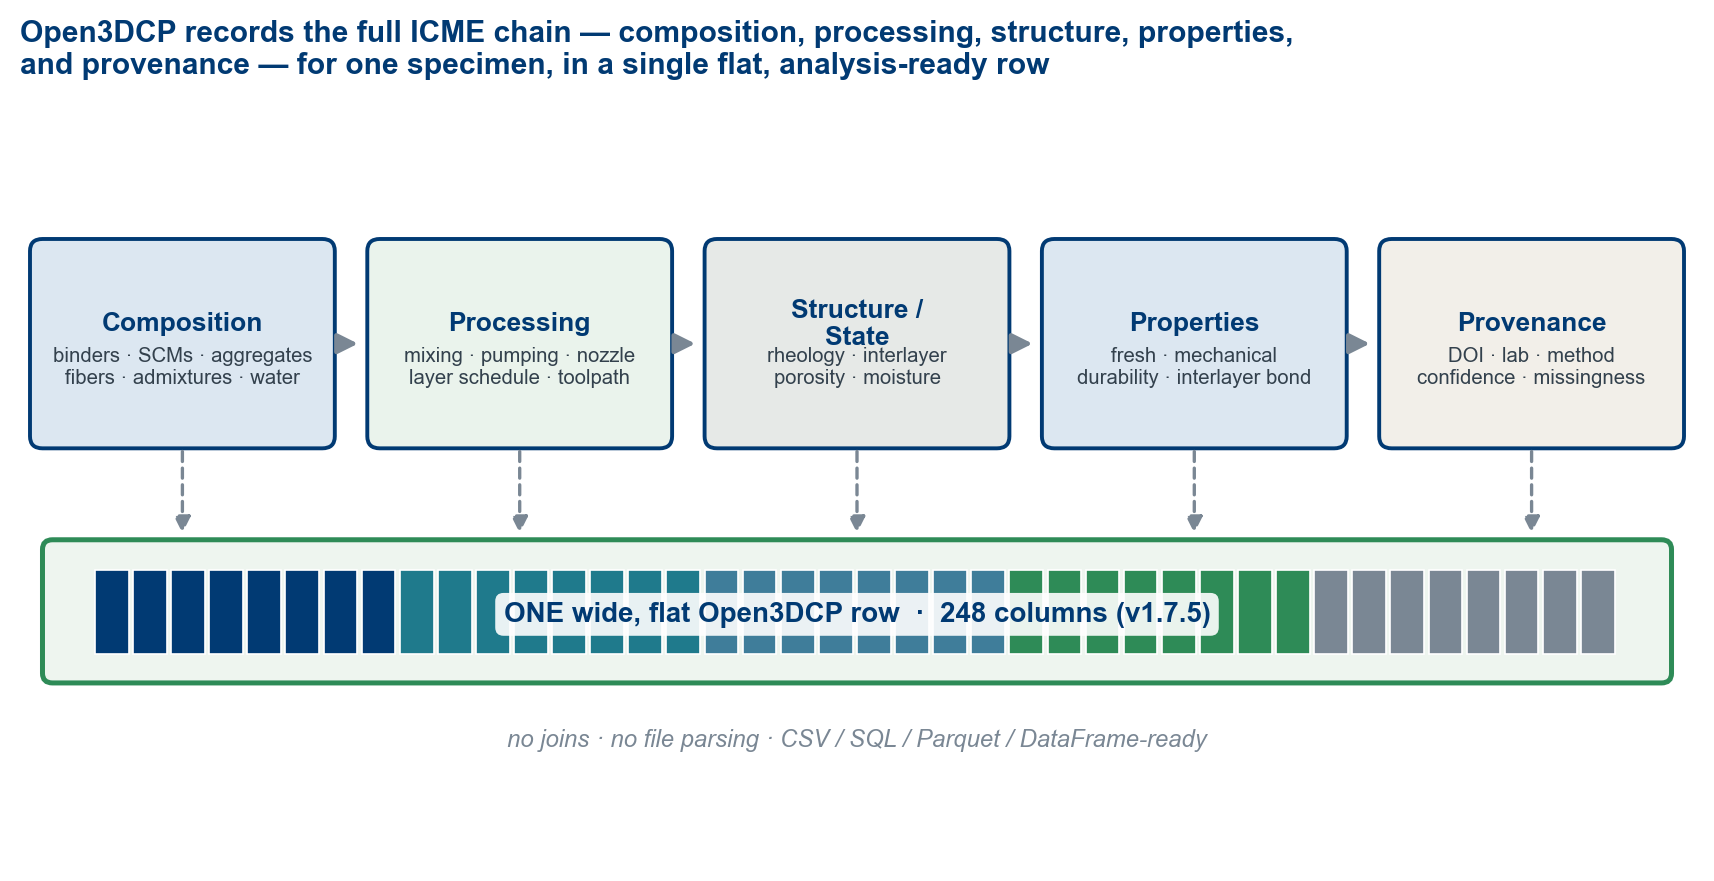
\includegraphics[width=6.2in,height=\textheight,keepaspectratio,alt={Open3DCP records the full ICME chain --- composition, processing, structure/state, properties, and provenance --- for one specimen in a single flat, analysis-ready row. The schema is the substrate for ICME-style process--structure--property analysis: it preserves the inputs and outcomes of a printed experiment without joins or file parsing.}]{figures/fig1_cppc_chain.png}
\caption{Open3DCP records the full ICME chain --- composition,
processing, structure/state, properties, and provenance --- for one
specimen in a single flat, analysis-ready row. The schema is the
substrate for ICME-style process--structure--property analysis: it
preserves the inputs and outcomes of a printed experiment without joins
or file parsing.}
\end{figure}

\begin{figure}
\centering
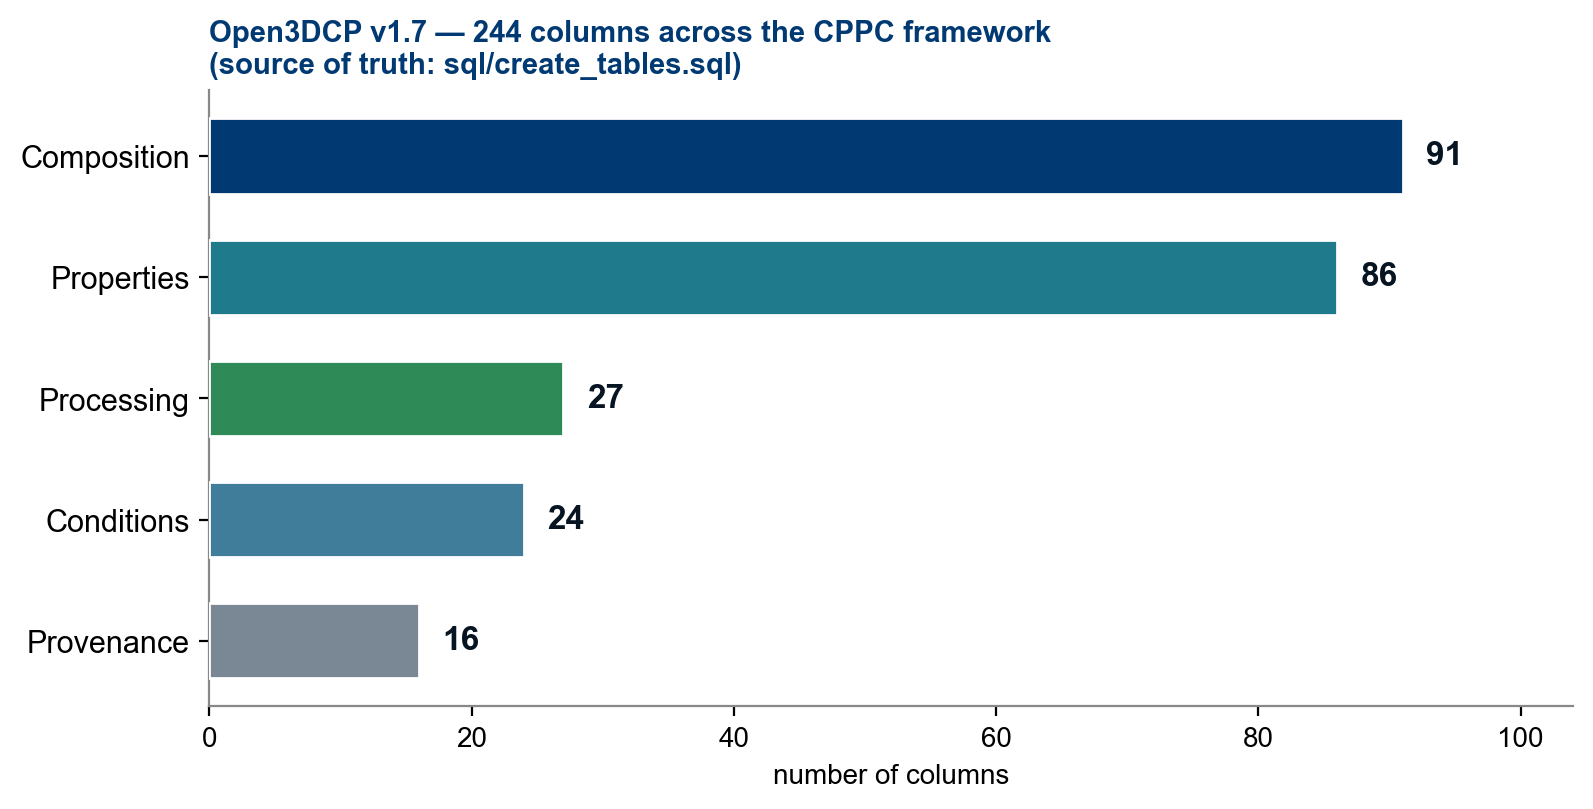
\includegraphics[width=5.6in,height=\textheight,keepaspectratio,alt={The 248 columns of Open3DCP v1.7.5 mapped to the CPPC framework. Counts are parsed from sql/create\_tables.sql, the schema's source of truth. Composition (95): binders, SCMs, activators, aggregates, fibers, admixtures, pigments, water, ratios, aggregate conditioning, basis and unspecified-constituent columns. Properties (86): fresh-state, mechanical, interlayer bond, durability, thermal, microstructure. Processing (27): 3DCP process parameters, pumping, mixing. Conditions (24): test conditions / specimen, environment, exposure class. Provenance (16): identity / versioning, source DOI, quality flags.}]{figures/fig2_column_inventory.png}
\caption{The 248 columns of Open3DCP v1.7.5 mapped to the CPPC
framework. Counts are parsed from
\protect\texttt{sql/create\_tables.sql}, the schema's source of truth.
\emph{Composition} (95): binders, SCMs, activators, aggregates, fibers,
admixtures, pigments, water, ratios, aggregate conditioning, basis and
unspecified-constituent columns. \emph{Properties} (86): fresh-state,
mechanical, interlayer bond, durability, thermal, microstructure.
\emph{Processing} (27): 3DCP process parameters, pumping, mixing.
\emph{Conditions} (24): test conditions / specimen, environment,
exposure class. \emph{Provenance} (16): identity / versioning, source
DOI, quality flags.}
\end{figure}

\begin{figure}
\centering
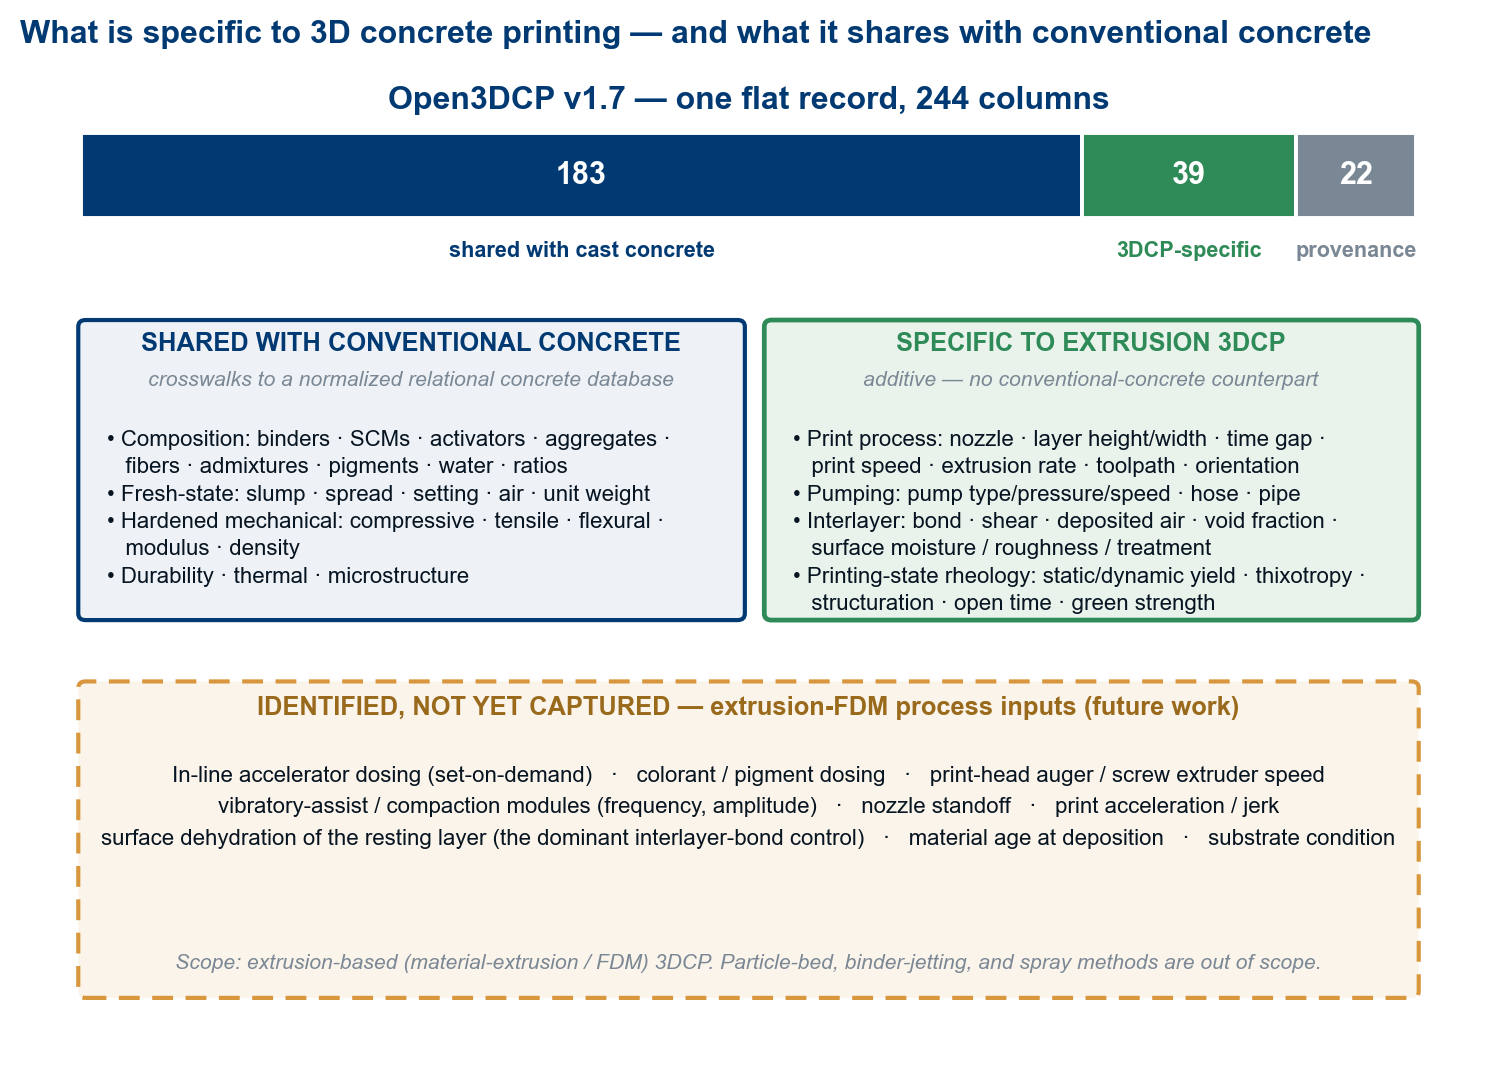
\includegraphics[width=6.3in,height=\textheight,keepaspectratio,alt={What is specific to 3D concrete printing, and what it shares with conventional concrete. Of the 248 columns, \textasciitilde187 describe composition and performance properties shared with cast concrete (and therefore crosswalk to a relational concrete database); \textasciitilde39 are specific to extrusion 3DCP (printing process, pumping, interlayer bond, printing-state rheology) with no conventional-concrete counterpart; the remaining \textasciitilde22 are provenance. (This is a different cut of the same 248 than the CPPC inventory in Figure 2 --- by origin rather than reporting role --- and also sums to 248.) The amber annex lists extrusion-process inputs identified but not yet captured --- a future-work agenda.}]{figures/fig3_data_classes.png}
\caption{What is specific to 3D concrete printing, and what it shares
with conventional concrete. Of the 248 columns, \textasciitilde187
describe composition and performance properties shared with cast
concrete (and therefore crosswalk to a relational concrete database);
\textasciitilde39 are specific to extrusion 3DCP (printing process,
pumping, interlayer bond, printing-state rheology) with no
conventional-concrete counterpart; the remaining \textasciitilde22 are
provenance. (This is a different cut of the same 248 than the CPPC
inventory in Figure 2 --- by origin rather than reporting role --- and
also sums to 248.) The amber annex lists extrusion-process inputs
identified but not yet captured --- a future-work agenda.}
\end{figure}

\begin{figure}
\centering
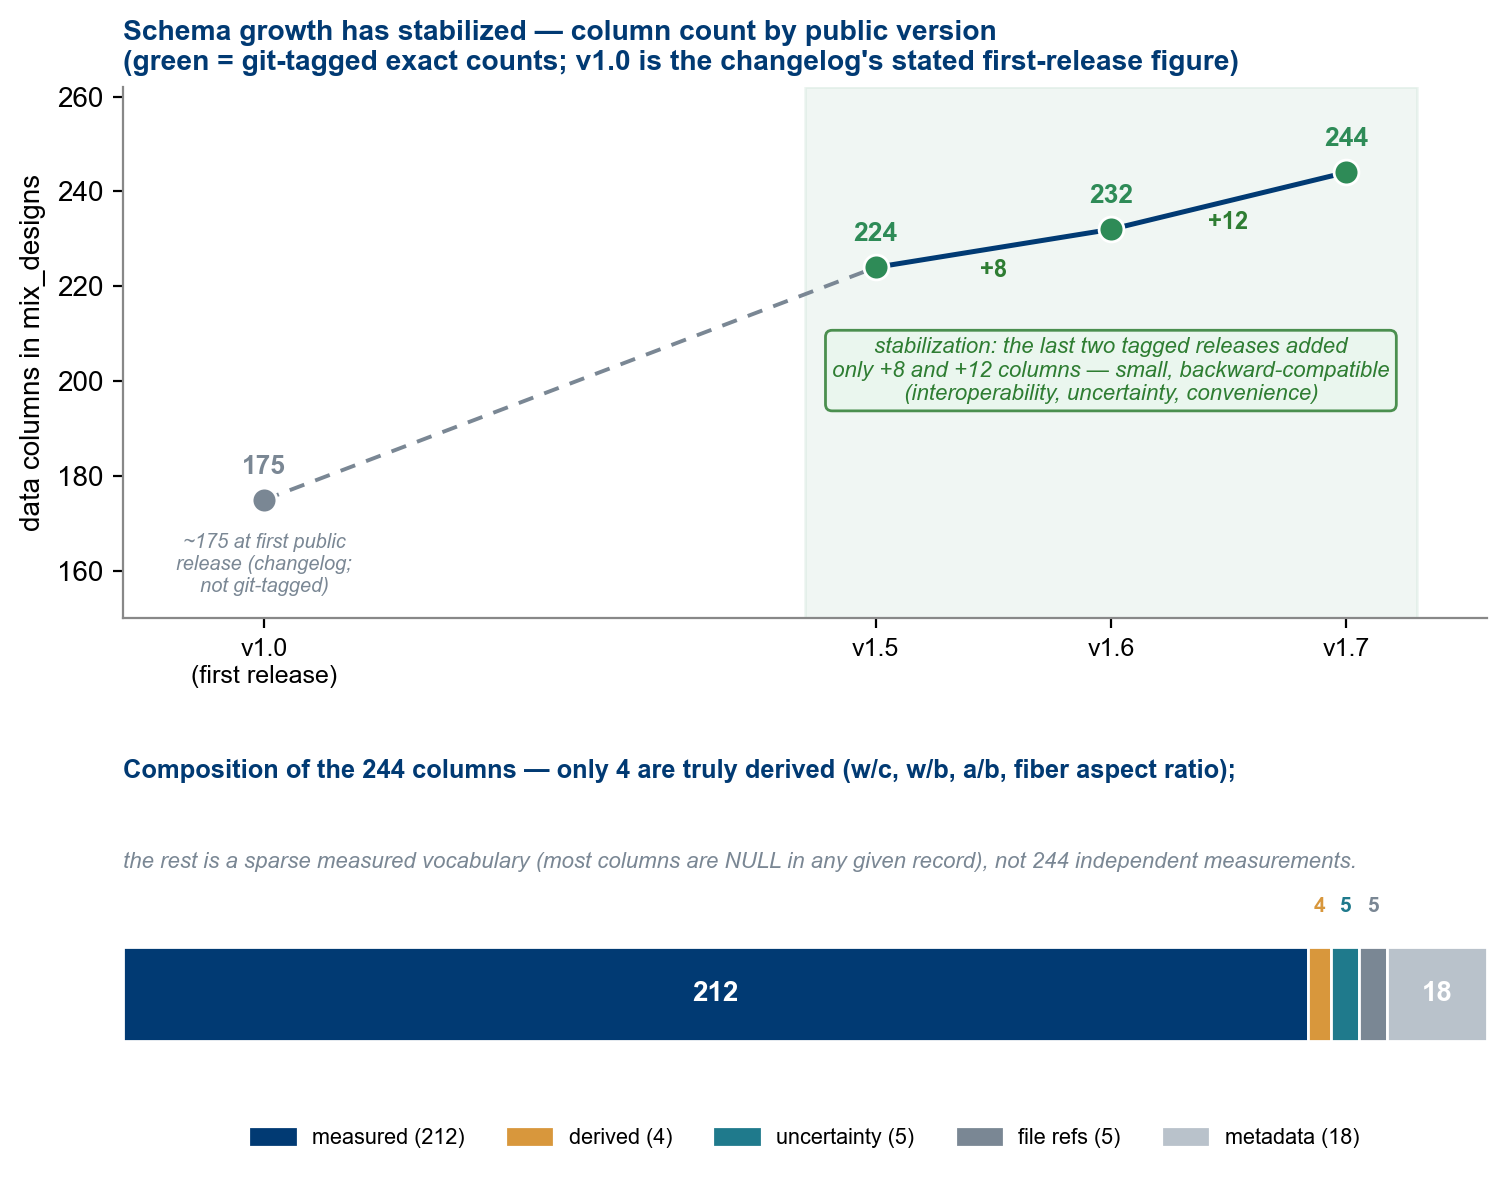
\includegraphics[width=5.8in,height=\textheight,keepaspectratio,alt={Schema growth has stabilized (top): v1.5 → v1.7.5 is a net +12 to 244 and then +4 to 248, and the only non-additive change across the tagged releases was the v1.6.5 SCM per-grade consolidation; the figure carries the per-release detail. Composition of the 248 (bottom): only four columns are derived from others, so the count is a sparse measured vocabulary --- the union of every reportable field, most NULL in any record --- not 248 independent measurements. Only the git-tagged releases (v1.5--v1.7.5) carry exact counts; v1.0 is the changelog's stated first-release figure (\textasciitilde175). The 248 are data columns, excluding the SERIAL primary key.}]{figures/fig4_schema_growth.png}
\caption{Schema growth has stabilized (top): v1.5 → v1.7.5 is a net +12
to 244 and then +4 to 248, and the only non-additive change across the
tagged releases was the v1.6.5 SCM per-grade consolidation; the figure
carries the per-release detail. Composition of the 248 (bottom): only
four columns are derived from others, so the count is a sparse measured
vocabulary --- the union of every reportable field, most NULL in any
record --- not 248 independent measurements. Only the git-tagged
releases (v1.5--v1.7.5) carry exact counts; v1.0 is the changelog's
stated first-release figure (\textasciitilde175). The 248 are data
columns, excluding the SERIAL primary key.}
\end{figure}

\textbf{Composition.} Portland and blended cements, calcium-aluminate
and calcium-sulfoaluminate cements, fly ash (generic, Class F, Class C
as separate columns per ASTM C618 oxide-sum classification), slag,
silica fume, metakaolin, limestone, pumice, bottom ash, rice-husk ash,
alkali activators, nanoscale modifiers, mineral powders, recycled sand,
pigments, aggregates, fibers, admixtures, clay rheology modifiers,
water, and derived ratios. The schema preserves chemically meaningful
distinctions rather than collapsing all cementitious material into a
single ``binder'' field, because fly-ash class, slag, silica fume,
limestone, and metakaolin are not interchangeable in hydration, packing,
rheology, or long-term performance.

\textbf{Fibers.} Eight core families --- \texttt{steel\_fiber},
\texttt{pp\_fiber}, \texttt{pva\_fiber}, \texttt{glass\_fiber},
\texttt{basalt\_fiber}, \texttt{carbon\_fiber}, \texttt{nylon\_fiber},
\texttt{aramid\_fiber} --- plus \texttt{cellulose\_fiber} for
natural-fiber compatibility (relevant to emerging 3DCP
wall-qualification frameworks such as ICC 1150 {[}47{]}), with geometry
captured separately (\texttt{fiber\_length\_mm},
\texttt{fiber\_diameter\_mm}, \texttt{fiber\_aspect\_ratio},
\texttt{fiber\_tensile\_strength\_mpa}). Aspect ratio is the single
strongest predictor of fiber contribution to post-crack toughness and is
rarely derivable from papers that report only type and dosage.

\textbf{Fresh-state and rheology.} Slump, spread, J-ring, V-funnel,
L-box, setting times, air content, fresh unit weight, bleeding, yield
stress (static and dynamic), plastic viscosity, thixotropy /
structuration rate, open time, and green strength. Printability is not a
single property: pumpability, extrudability, shape stability, and open
time can move in different directions as water, superplasticizer, VMA,
accelerator, grading, and ambient conditions change.

\textbf{Process parameters.} Print speed, layer height and width, layer
time gap, nozzle diameter / shape / area, filament width, extrusion
rate, number of layers, path length, infill pattern, contour count,
print direction, and pumping/mixing/environmental conditions --- the
processing leg of the ICME chain, absent from prior concrete datasets.
The process columns and their typical downstream outcomes are specified
in the repository.

\textbf{Specimen and test context.} Specimen preparation, geometry,
dimensions, extraction method, curing conditions, test age, test method,
number of specimens averaged, and \textbf{test orientation} ---
especially important because printed concrete is anisotropic.
Orientation is a controlled vocabulary (Table 1).

{\def\LTcaptype{none} % do not increment counter
\begin{longtable}[]{@{}
  >{\raggedright\arraybackslash}p{(\linewidth - 6\tabcolsep) * \real{0.2500}}
  >{\raggedright\arraybackslash}p{(\linewidth - 6\tabcolsep) * \real{0.2500}}
  >{\raggedright\arraybackslash}p{(\linewidth - 6\tabcolsep) * \real{0.2500}}
  >{\raggedright\arraybackslash}p{(\linewidth - 6\tabcolsep) * \real{0.2500}}@{}}
\toprule\noalign{}
\begin{minipage}[b]{\linewidth}\raggedright
Code
\end{minipage} & \begin{minipage}[b]{\linewidth}\raggedright
Axis
\end{minipage} & \begin{minipage}[b]{\linewidth}\raggedright
Description
\end{minipage} & \begin{minipage}[b]{\linewidth}\raggedright
Typical strength*
\end{minipage} \\
\midrule\noalign{}
\endhead
\bottomrule\noalign{}
\endlastfoot
\texttt{X} & Longitudinal & Parallel to extrusion direction (along the
print path) & Highest \\
\texttt{Y} & Transverse & Perpendicular, within layer plane &
Moderate \\
\texttt{Z} & Interlayer & Perpendicular to layer interfaces (build axis)
& Lowest \\
\texttt{XY\_45} & In-plane & 45° diagonal in layer plane & X--Y
intermediate \\
\texttt{XZ\_45} & Cross-layer & 45° diagonal across layers & X--Z
intermediate \\
\texttt{CAST} & Isotropic & Moulded reference specimen & Baseline \\
\end{longtable}
}

* Indicative ordering for \textbf{axial (compressive) loading}, and
mix-dependent. In \textbf{flexure} the ordering can invert: loading
along the print path (\texttt{X}) bends the interlayer planes in
tension, so \texttt{X} is typically the \emph{weakest} flexural
orientation --- exactly what the worked demonstration measures later in
this section.

Table: Test-orientation controlled vocabulary. Strength ordering is
typical; specific values depend on mix design and process parameters
{[}5, 6{]}.

\textbf{Hardened, durability, and interlayer.} Compressive, tensile,
splitting tensile, flexural, modulus, bond, fracture energy, toughness,
impact, fatigue, density, and Poisson's ratio; a durability suite
covering chloride transport, carbonation, shrinkage, creep,
freeze--thaw, sulfate and ASR expansion, permeability, absorption,
sorptivity, scaling, corrosion indicators, thermal properties, and fire
resistance; and interlayer columns for bond, shear, void-area fraction,
deposited air content, surface roughness, surface moisture state, and
surface treatment. The schema does not assert that every dataset
measures all of these; it provides stable homes when the measurements
exist.

\textbf{Provenance, basis, and uncertainty.} Beyond DOI, citation,
confidence, lab, and quality flags, v1.7 added per-measurement
uncertainty columns (e.g.~\texttt{compressive\_strength\_stddev\_mpa}),
raw-data references that keep large payloads external
(\texttt{raw\_data\_doi}, \texttt{stress\_strain\_file},
\texttt{rheology\_curve\_file}, \texttt{microstructure\_image},
\texttt{raw\_data\_file}), the basis columns of §5.2, a
\texttt{material\_class} classification, a batch timeline
(\texttt{batch\_label}, \texttt{date\_of\_casting}), and
aggregate-conditioning columns (\texttt{aggregate\_moisture\_state},
\texttt{aggregate\_absorption\_pct},
\texttt{aggregate\_moisture\_content\_pct},
\texttt{aggregate\_prewetted}) that make effective mix water recoverable
when aggregates are batched off the SSD reference.

\textbf{Quantifying the cost of flattening.} Projecting a heterogeneous
or relational source onto one flat row can lose information. Rather than
hide that, the fidelity of the mapping can be scored against the source
and reported --- a proposed, not-yet-calibrated convention (§10) --- so
the cost of each conversion is recorded rather than hidden. A
machine-readable crosswalk to a normalized relational concrete database,
and a specification of the process-parameter columns that have no
conventional relational counterpart, are included in the repository.

\textbf{Worked demonstration: five public datasets in one schema.} To
show the schema works on real data --- not only by design --- we
ingested five openly-licensed public datasets into Open3DCP, chosen so
that each lights up a \emph{different} slice of the record (Figure 5,
left). Two are flat kg/m³ tables that the \texttt{open3dcp-ingest} tool
converts and scores automatically:

\begin{itemize}
\tightlist
\item
  \textbf{UCI/Yeh (1998)} {[}4{]}, a \emph{cast}-concrete benchmark,
  maps onto composition and hardened strength and ingests at
  \textbf{100/100 (A)} (126 populated cells across its 9 source fields)
  with \textbf{zero assumptions}: every constituent mass is stored
  exactly, and the four details the source never records --- the cement
  type, the fine- and coarse-aggregate gradations, and the
  superplasticizer solids fraction --- are stored \emph{generically}
  (the \texttt{*\_unspecified} columns and the \texttt{admixture\_basis}
  flag) with the classification left NULL rather than guessed. The
  fidelity report discloses those 47 generically-recorded cells
  alongside the score. It remains the normal-strength reference point.
\item
  \textbf{Meta SustainableConcrete} {[}49{]}, an openly-licensed (MIT)
  carbon-aware set from Meta with the University of Illinois and Amrize,
  ingests at \textbf{100/100 (A)} on the same terms and additionally
  populates \textbf{embodied carbon} (per-mix global warming potential,
  GWP) and the measurement-uncertainty columns. It makes a cross-source
  trade-off legible in one schema: a plain-Portland concrete (Mix\_84)
  at \textasciitilde521 kg CO\textsubscript{2}/m³ for \textasciitilde65
  MPa beside a low-clinker ternary (Mix\_88) at \textasciitilde204 kg
  CO\textsubscript{2}/m³ for \textasciitilde110 MPa --- a low-clinker
  binder reaching high strength at a fraction of the embodied carbon.
  (The strength gap also reflects a lower water/binder ratio --- 0.25 vs
  0.40; a second mix at the \emph{same} \textasciitilde204 kg
  CO\textsubscript{2}/m³ reaches \textasciitilde61 MPa --- one
  illustrative pair, not a carbon-drives-strength trend. Where dosages
  are design proportions that do not close a 1 m³ batch, the ingest tool
  flags the row in \texttt{provenance\_notes} and per-m³ quantities
  inherit the discrepancy; the repository's \emph{model-generated}
  candidate mixes, kept distinct from measured data by
  \texttt{measurement\_confidence}, are a natural next ingestion, not
  attempted here.)
\end{itemize}

These scores are an honest \emph{ingestion-fidelity} check on a curated
excerpt, not a dataset-quality grade. The metric scores only the
dimensions a flat source can actually exercise --- relational-integrity
and file-capture are reported \emph{not applicable} and excluded rather
than credited a free 100 --- renormalizes over those, and \textbf{caps
the grade by its weakest applicable dimension}, so near-complete field
coverage cannot float a low value-fidelity to an ``A''. Value-fidelity
counts every cell that rests on a genuine assumption (a guessed solids
fraction or product density, a volume dose without one, an
incomplete-batch projection) against the cells stored exactly. The
metric earned its keep against this very schema: an earlier draft
\emph{defaulted} unstated classifications --- a cement type, two
aggregate gradation buckets --- and the metric priced those guesses at
\textbf{79.9/C} for UCI. Rather than accept fabricated certainty,
\textbf{v1.7.5 added the \texttt{*\_unspecified} columns and the
\texttt{admixture\_basis} flag} described in the UCI entry above, and
the same data then ingests with zero assumptions. A perfect score
therefore means precisely ``nothing was assumed'' --- and the report
still lists every generically-recorded cell --- while messy sources
(volume doses, missing batch masses, unstated units) are penalized
exactly as before. The convention is documented in §10, deliberately
conservative, and not yet calibrated against a labelled benchmark.

Three more are curated through their native structure (a fidelity score
for each awaits a dedicated reader, exactly as the tool is extended
source by source):

\begin{itemize}
\tightlist
\item
  The \textbf{RILEM TC 304-ADC} interlaboratory study on the mechanical
  properties of 3D-printed concrete {[}48{]} --- a \emph{real 3DCP}
  database from roughly thirty laboratories, stored as a normalized
  relational SQLite export --- populates 3DCP process, fresh-state
  rheology, hardened mechanical, \textbf{orientation}, and the
  per-measurement uncertainty columns (mean ± standard deviation ± n).
\item
  The \textbf{University of Florida 3D-Printing-Concrete Mix-Design}
  dataset {[}50{]} supplies the extrusion-3DCP \emph{printability} slice
  --- static and dynamic yield stress and plastic viscosity --- and is
  an honest illustration of a basis mismatch: it reports constituents as
  ratios to binder with no absolute kg/m³, so a constituent mass-\% of
  the mix is left NULL rather than invented.
\item
  The \textbf{TU-Braunschweig Database of 3D Concrete Printed Buildings}
  {[}51{]} supplies the \emph{project / process layer} --- as-built
  printed structures by consortium, country, and system --- a slice with
  no mix or strength data, which the current mix-centric schema records
  as provenance and marks as the frontier a future project/process table
  will type.
\end{itemize}

A UHPC source surveyed for this work, the Stevens dataset (Mahjoubi \&
Bao), was excluded as reference-only: its mix variables are published as
a coded ML feature matrix whose legend is paywalled, so it cannot be
honestly re-ingested. Together the five light up complementary slices,
and Open3DCP holds the union of these five sources in one shape --- and
\emph{the empty cells are as much the point as the full ones}: what each
source cannot supply is recorded, not hidden (Figure 5, left).

The demonstration also yields a characterization result that
\textbf{cannot be expressed without an orientation field, nor compared
across laboratories without a shared schema}: print anisotropy. Mapping
the RILEM U/V/W loading codes onto Open3DCP's
\texttt{test\_orientation\_code} (X/Y/Z/CAST), printed concrete loaded
\textbf{along the print path is 32--55 \% weaker in flexure} than its
cast reference in each of three independent single-lab datasets ---
three \emph{different} commercial premixes tested at
\textasciitilde28--30 days (per-lab reductions 40 \%, 32 \%, and 55 \%;
n = 12--40 per group). The reductions agree in direction across all
three, but the datasets share no formulation, so this is a consistent
single-lab observation rather than a pooled estimate; the 55 \% upper
bound is the least-pinned, resting on a 12-specimen cast group with
\textasciitilde40 \% coefficient of variation (roughly ± 7 percentage
points of standard error). Literature reductions for specimens loaded
\emph{across} the layer interface run \textasciitilde20--40 \% {[}5,
6{]}; our along-path \emph{flexural} reductions run higher because
bending concentrates tension on the interlayer planes. (That is also why
Table 1's ``typical strength'' ordering --- stated for axial loading ---
inverts here, as the table note and Limitation 4 say.) This is a
demonstration of \emph{ingestion and interoperability} --- recording
what was measured in one comparable shape --- not a predictive-model
benchmark; assembling and modelling a pooled multi-source corpus is
future work (§11).

\begin{figure}
\centering
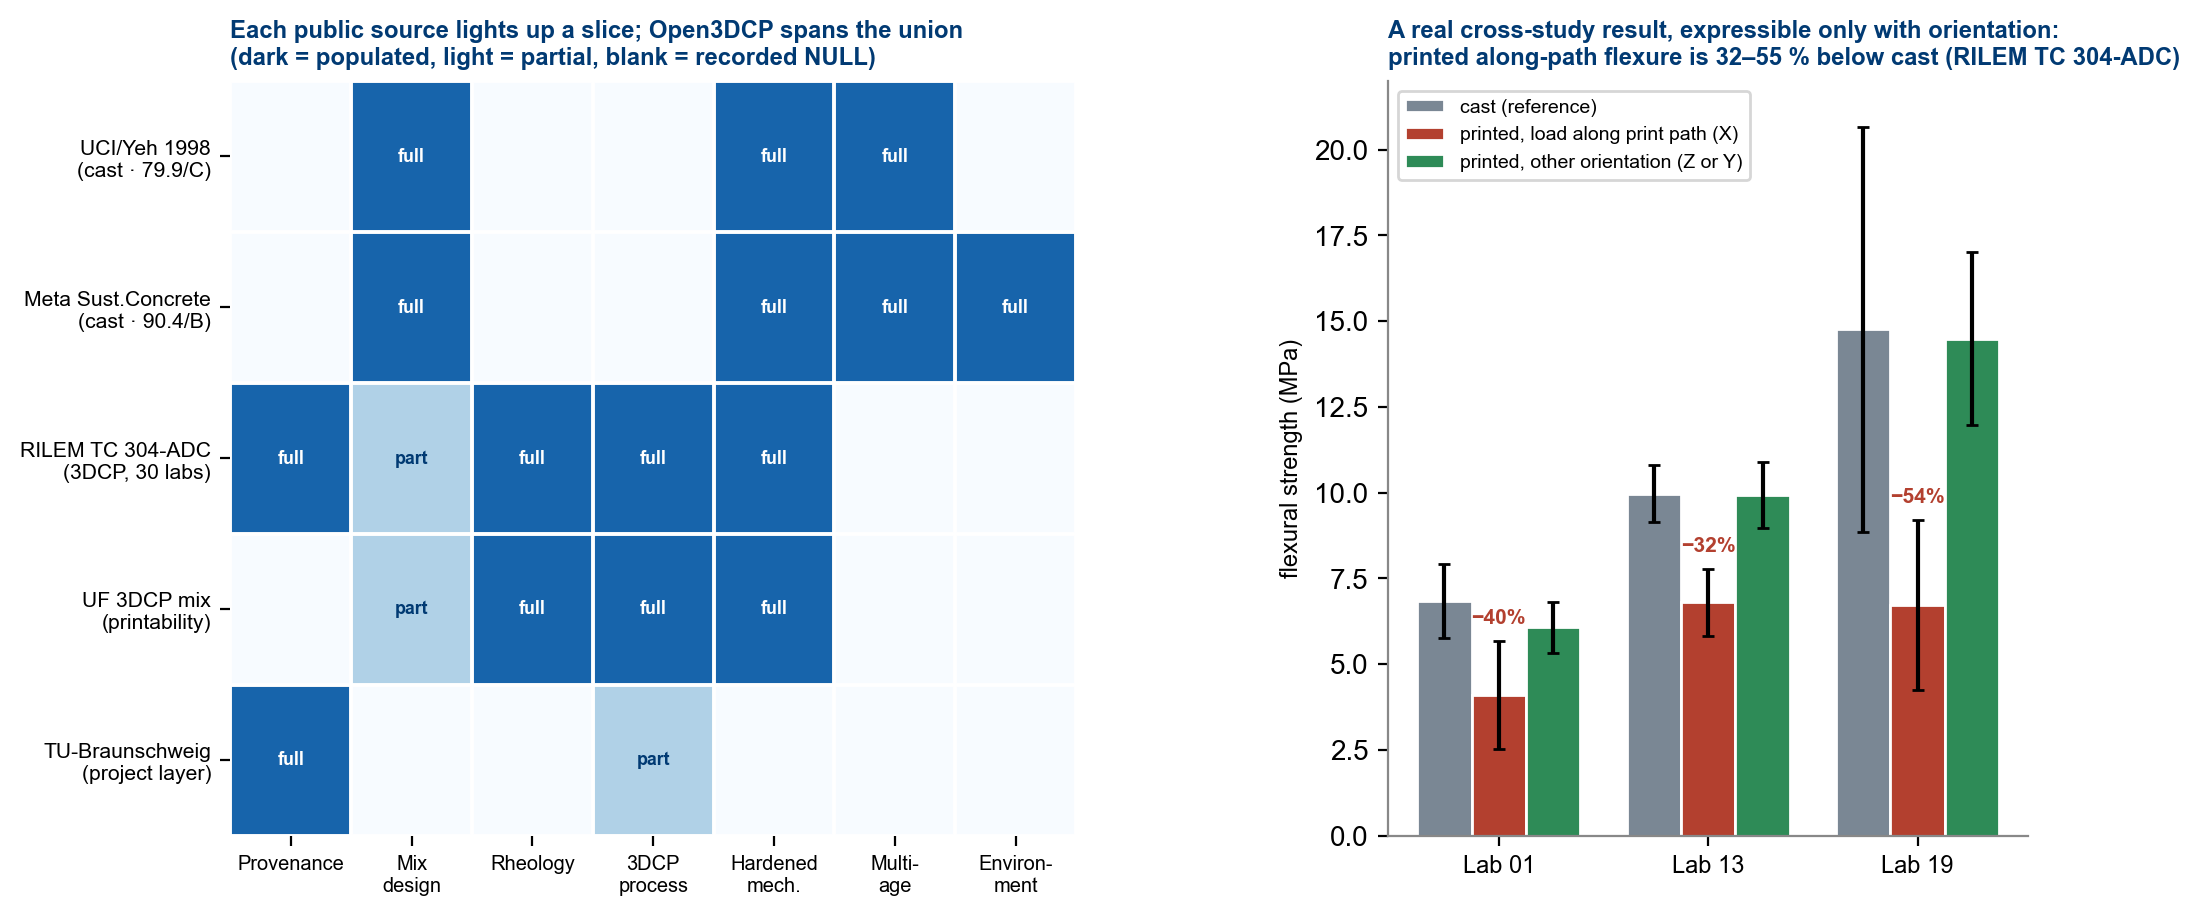
\includegraphics[width=6.4in,height=\textheight,keepaspectratio,alt={Worked demonstration. Left: five openly-licensed public datasets ingested into Open3DCP --- UCI/Yeh (cast benchmark), Meta SustainableConcrete (cast, carbon-aware), the RILEM TC 304-ADC interlaboratory study (real 3DCP, \textasciitilde30 labs), the UF 3DCP mix-design set (printability), and the TU-Braunschweig 3DCP buildings catalogue (project layer) --- each populating a different slice of the record (dark = populated, light = partial/absent), with Open3DCP spanning the union; the empty cells are recorded, not hidden. The two flat kg/m³ sources carry an automated open3dcp-ingest fidelity score (both 100/A --- zero assumptions, with generically-recorded cells disclosed; see §6); the rest are curated through their native structure. Right: a cross-study characterization result from the RILEM data, expressible only because the schema records loading orientation --- printed concrete loaded along the print path (X) is 32--55 \% weaker in flexure than the cast reference in three independent single-lab datasets (three different premixes, \textasciitilde28--30 d, per-lab n = 12--40; error bars are ± one standard deviation).}]{figures/fig5_demonstration.png}
\caption{\textbf{Worked demonstration.} \emph{Left:} five
openly-licensed public datasets ingested into Open3DCP --- UCI/Yeh (cast
benchmark), Meta SustainableConcrete (cast, carbon-aware), the RILEM TC
304-ADC interlaboratory study (real 3DCP, \textasciitilde30 labs), the
UF 3DCP mix-design set (printability), and the TU-Braunschweig 3DCP
buildings catalogue (project layer) --- each populating a different
slice of the record (dark = populated, light = partial/absent), with
Open3DCP spanning the union; the empty cells are recorded, not hidden.
The two flat kg/m³ sources carry an automated
\protect\texttt{open3dcp-ingest} fidelity score (both 100/A --- zero
assumptions, with generically-recorded cells disclosed; see §6); the
rest are curated through their native structure. \emph{Right:} a
cross-study characterization result from the RILEM data, expressible
only because the schema records loading orientation --- printed concrete
loaded along the print path (X) is 32--55 \% weaker in flexure than the
cast reference in three independent single-lab datasets (three different
premixes, \textasciitilde28--30 d, per-lab n = 12--40; error bars are ±
one standard deviation).}
\end{figure}

\subsection{7. Digital twin and ICME
framing}\label{digital-twin-and-icme-framing}

A full digital twin of a 3DCP process spans at least four layers of
information: a \textbf{material definition} (composition, product
identity, particle characteristics, water/admixture basis, fiber
geometry); a \textbf{process definition} (mixing, pumping, nozzle
geometry, motion, extrusion rate, layer schedule, environment, curing);
\textbf{state and structure} (fresh rheology, thixotropic recovery,
interlayer surface condition, porosity, moisture, temperature,
hydration, fiber orientation, microstructure); and \textbf{performance
and provenance} (mechanical and durability properties, test method,
specimen geometry, orientation, lab, confidence, source). Open3DCP
covers much of the first, second, and fourth, and a useful subset of the
third (Figure 1). \textbf{Open3DCP is not a digital twin.} A digital
twin, as the digital-fabrication community uses the term, requires live,
bidirectional coupling to the running process; a static, scalar,
single-row schema has none. Open3DCP is better described as a
\emph{structured experiment record} --- a substrate from which many
aspects of published 3DCP work can be reconstructed and compared, and on
which future digital twins could be built. Full process twins will
additionally require time-series machine logs, synchronized sensor data,
imaging, and richer links to raw files.

\subsection{8. What we cannot capture --- and
why}\label{what-we-cannot-capture-and-why}

This section identifies features that are physically important for 3DCP
but cannot currently be measured reliably. The taxonomy is intended to
guide instrumentation research and future schema extensions, not to
claim the schema is complete.

\textbf{8.1 Real-time process-monitoring gaps.} The schema stores
rheology as point measurements (typically a pre-print laboratory
rheometer reading), but the material's rheological state changes
continuously from mixer through pump, hose, and nozzle; no inline
rheometer exists for cementitious materials at production scale. Pump
pressure is a single scalar, yet in practice it fluctuates with
consistency and toolpath back-pressure in ways that correlate with
segregation and flow discontinuities. Nozzle standoff is a nominal value
that varies with robot positioning and substrate deformation. And
print-head dynamics --- acceleration, deceleration, cornering --- cause
local variation in deposition rate not captured by a single print-speed
value.

\textbf{8.2 In-situ material-state gaps.} The actual interlayer moisture
at the moment of deposition is a continuous field depending on ambient
humidity, wind, time gap, and diffusivity; Sanjayan et al.~{[}8{]}
showed it affects bond by 20--40 \% and Moelich et al.~{[}9{]} modeled
it quantitatively, yet no standardized protocol measures it in
production. The degree of hydration at each interface forms a gradient
across layers, but the schema stores a single destructively-measured
value. Fiber-orientation distribution critically affects directional
strength but can only be measured destructively by micro-CT after
hardening. Aggregate packing within the filament and the internal
temperature field during exothermic curing are likewise not measurable
in-situ.

\textbf{8.3 Characterization-protocol gaps.} Interlayer void fraction
requires destructive cross-sectional imaging with no standardized
analysis; surface roughness at layer interfaces has no standard protocol
for 3DCP; and ambient conditions reported as room averages may differ
from the point of deposition in large-scale or outdoor printing.

\textbf{8.4 Process inputs not yet captured.} Beyond the real-time
signals above, several extrusion-process \emph{inputs} an operator sets
are not yet schema columns. The priority gap is \textbf{in-line
accelerator dosing at the print head} (set-on-demand): on dosing-pump
systems it is the control variable an operator tunes to keep the print
standing, and a record without it omits the knob that most directly sets
buildability --- today only \texttt{admixture\_addition\_point} and the
bulk \texttt{accelerator} column hint at it. Next in line:
\textbf{material age at deposition and on-site retempering} (water or
admixture added as the hopper ages, which silently moves the
as-deposited w/b away from the batch ticket), print-head auger / screw
extruder speed (distinct from the bulk-mixer speed the schema records),
colorant / pigment dosing, and vibratory-assist or compaction modules
--- alongside nozzle standoff, print acceleration / jerk, and surface
dehydration of the resting layer (the dominant interlayer-bond control)
(Figure 3, annex). These are an explicit future-work agenda; the schema
extends additively as they are specified.

\textbf{8.5 The digital-twin horizon.} A complete twin would require on
the order of 300+ parameters, including time-series data that cannot be
represented as scalar columns. Open3DCP captures the formulation,
process, and performance layers of a record well, plus a useful part of
the in-situ state layer; the largest remaining gap is the real-time
process data that current hardware does not routinely capture. As sensor
technology improves --- inline rheometers, thermal imaging tied to
print-head motion, machine vision for filament geometry --- the flat
schema can extend additively without breaking existing queries. The gap
analysis is not a criticism of the schema's completeness: \textbf{the
features we cannot measure today are, in many cases, the features that
most limit a complete characterization of the printed material}, and
closing these gaps requires instrumentation, not schema design.

\subsection{9. Adoption path and
community}\label{adoption-path-and-community}

Adoption does not require populating every column --- null columns are
ignored during analysis. A laboratory can adopt the schema by (1)
mapping local column names to canonical Open3DCP names; (2) recording
material quantities with the source basis preserved
(\texttt{original\_basis}) so kg/m³ ↔ mass-percent remains exact; (3)
preserving missing values as \texttt{NULL} and using \texttt{0} only for
explicit zeros; (4) filling provenance fields before analysis fields;
(5) recording test method, specimen geometry, age, and orientation for
every mechanical result; (6) depositing the dataset in a public
repository when rights allow; and (7) citing the schema and the original
test methods. The flat schema is database-agnostic (PostgreSQL, SQLite,
CSV, Parquet, pandas/polars/R) and pairs naturally with standard ML
libraries for an end-to-end, open-source pipeline. By design it is
\textbf{FAIR-aligned} {[}18{]}: every record carries a DOI or citation
(Findable), the schema is open under Apache-2.0 (Accessible), naming
follows ASTM/EN/RILEM with SI units and controlled vocabularies
(Interoperable), and the license plus provenance metadata supports reuse
(Reusable).

Because most of the schema is shared with conventional concrete (§6),
Open3DCP interoperates closely with a normalized relational concrete
database (Figure 6). Material composition and test results map both ways
--- exactly for ages, geometry, and ratios; with a recorded density for
the kg/m³ ↔ mass-percent step. The correlation is close but the
round-trip is \emph{not} lossless: relational structure that a flat row
cannot hold (parametrized geometry, reinforcement layouts, devices,
loading histories) collapses to a side record, and the extrusion-3DCP
process and interlayer columns have no conventional relational table to
map into. Stating these boundaries is what makes the mapping auditable
rather than asserted.

\begin{figure}
\centering
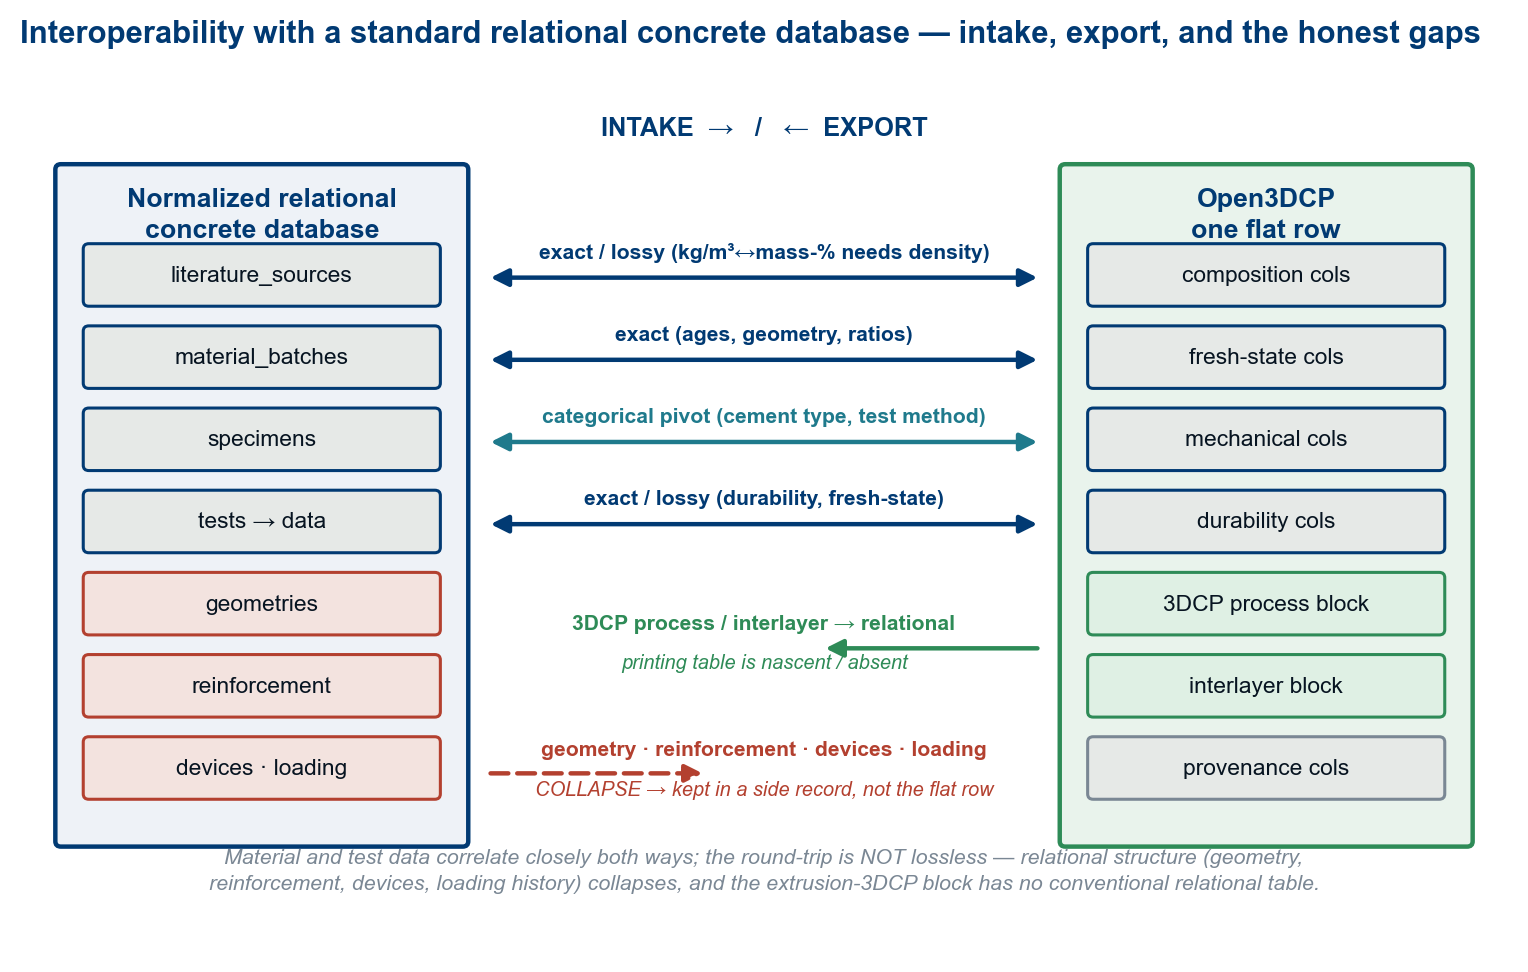
\includegraphics[width=6.2in,height=\textheight,keepaspectratio,alt={Interoperability with a normalized relational concrete database. Material and test data map both ways by fidelity class (exact / lossy / categorical); the round-trip is not lossless --- relational structure (geometry, reinforcement, devices, loading history) collapses to a side record, and the extrusion-3DCP block has no conventional relational counterpart.}]{figures/fig6_crosswalk.png}
\caption{Interoperability with a normalized relational concrete
database. Material and test data map both ways by fidelity class (exact
/ lossy / categorical); the round-trip is not lossless --- relational
structure (geometry, reinforcement, devices, loading history) collapses
to a side record, and the extrusion-3DCP block has no conventional
relational counterpart.}
\end{figure}

We invite the 3DCP community to adopt common column names and units in
published datasets --- even partial adoption of shared names for fields
like \texttt{compressive\_strength\_mpa}, \texttt{w\_b\_ratio},
\texttt{layer\_height\_mm}, and \texttt{test\_orientation\_code} would
sharply reduce the effort of combining datasets --- and we encourage
standards bodies and the community to evaluate Open3DCP (or a
derivative) as one input to future 3DCP data-reporting practice,
extending the RILEM TC 304-ADC database approach {[}14{]} from
interlaboratory studies to routine publication.

\subsection{10. Limitations}\label{limitations}

These limitations bound the claims above; §11 maps each to planned work.

\begin{enumerate}
\def\labelenumi{\arabic{enumi}.}
\tightlist
\item
  \textbf{Coverage is a v1.7.5 snapshot.} The 248-column count and
  per-category figures reflect \texttt{sql/create\_tables.sql} at
  v1.7.5; the schema is under active, additive development and these
  numbers evolve. The canonical reference is always the repository.
\item
  \textbf{Single-maintainer governance and unquantified curation
  reliability.} The schema and its controlled vocabularies are
  maintained by one author; column choices and any scoring conventions
  are an expert convention, not yet ratified by a working group or
  calibrated against a labelled benchmark. The reliability of human
  curation --- \texttt{NULL}-vs-\texttt{0} judgements, confidence flags,
  basis assignment, and the resolution of conflicting or duplicate
  source values --- is likewise not yet quantified (no inter-curator
  agreement study).
\item
  \textbf{The measurement-gap taxonomy is qualitative.} §8 names gaps
  and their physical importance but does not quantify how much each
  would improve a model; that ordering awaits feature-ablation studies
  on datasets built with the schema.
\item
  \textbf{Typical ranges and orientation orderings are indicative}, not
  gates, and not yet sourced to a fixed citation set; Table 1's strength
  ordering is typical, not measured here.
\item
  \textbf{Adoption at scale is unproven, and pooled modeling carries
  stated traps.} Cross-dataset interoperability is asserted by design;
  no large, heterogeneous, multi-source corpus has yet been assembled
  and modeled end-to-end on the public schema --- the committed
  demonstration totals roughly seventy rows across five sources, an
  interoperability proof, not a trainable corpus. Anyone pooling records
  should treat the source/laboratory as a covariate (premixes, specimen
  geometries, and protocols differ across sources --- a textbook
  confounding setup), and should note that several columns are
  \emph{records}, not model features: \texttt{design\_strength\_mpa}
  leaks the strength target, the derived ratios are collinear with their
  inputs, and the dual-basis pair encodes the same composition twice.
  The quality flags (\texttt{is\_training\_ready},
  \texttt{is\_synthetic}, \texttt{outlier\_flag}) are defined but
  deliberately not set in the demonstration excerpts; the quality gate
  that sets them is future work.
\item
  \textbf{The schema is not a substitute for validation.} It records
  what was done and measured; it does not certify structures, validate
  models, or establish that a mix is printable, durable, or safe.
\end{enumerate}

\subsection{11. Future work}\label{future-work}

\begin{enumerate}
\def\labelenumi{\arabic{enumi}.}
\tightlist
\item
  Assemble and publish a \textbf{multi-source corpus} on the public
  schema and report cross-dataset model performance and the
  data-coverage distribution across the CPPC categories.
\item
  \textbf{Validate the source-to-schema mapping} --- tie any fidelity
  scoring of the mapping to a labelled benchmark or a measured
  downstream consequence, and add a sensitivity analysis.
\item
  \textbf{Quantify the measurement gaps} of §8 through feature-ablation
  studies, converting the qualitative taxonomy into a ranked
  instrumentation agenda.
\item
  Move governance toward a \textbf{working-group / standards process}
  (with RILEM, ACI, or ASTM) so the vocabulary and grade bands are
  community-ratified rather than single-author conventions.
\item
  Extend additively as instrumentation matures (inline rheometry,
  thermal imaging, machine vision), keeping the flat-schema
  backward-compatibility guarantee.
\item
  Calibrate and extend the \textbf{machine-readable crosswalk package}
  now in the repository alongside the relational-database crosswalk ---
  mappings to AM-CDM {[}52{]}, GEMD {[}59{]}, and PMDco/CPTO {[}54,
  55{]} with field-level mapping classes (exact / normalized / derived /
  partial / sidecar / no\_map) and pinned target versions: complete the
  per-mapping notes, assign the reserved sidecar class as the
  linked-record sidecars land, and re-pin targets as they release.
\end{enumerate}

\subsection{12. Data and code
availability}\label{data-and-code-availability}

\begin{itemize}
\tightlist
\item
  \textbf{Schema \& tooling:} Open3DCP v1.7.5 {[}45{]} ---
  \texttt{github.com/sunnyday-technologies/Open3DCP} (Apache-2.0);
  Zenodo concept DOI \texttt{10.5281/zenodo.19647470} (resolves to the
  latest \emph{published} Zenodo version --- currently v1.6.0; the v1.7
  described here is the working draft pending its Zenodo release). The
  canonical column list is \texttt{Open3DCP\_SCHEMA.md} /
  \texttt{sql/create\_tables.sql}; companion tables include
  \texttt{strength\_measurements}, \texttt{sources},
  \texttt{test\_methods}, \texttt{curing\_regimes}, and
  \texttt{material\_aliases}.
\item
  \textbf{Reproducing the figures:} the column counts in Figures 2 and 4
  are parsed from \texttt{sql/create\_tables.sql}, the schema's single
  source of truth; the figures are regenerated by the committed figure
  scripts (matplotlib, PNG ≥ 200 dpi + SVG).
\item
  \textbf{Supporting material:} machine-readable crosswalks --- to a
  normalized relational concrete database
  (\texttt{crosswalk/open3dcp\_to\_relational.yaml}) and to the AM-CDM,
  GEMD, and CPTO data models
  (\texttt{crosswalk/open3dcp\_to\_amcdm.csv}, \texttt{\_gemd.csv},
  \texttt{\_cpto.csv}) --- and a specification of the 3DCP
  process-parameter columns are included in the repository.
\end{itemize}

\subsection{13. Manuscript license and author
statements}\label{manuscript-license-and-author-statements}

\textbf{Manuscript license.} Copyright © 2026 Sunnyday Technologies LLC
and Nicholas Sonnentag. This manuscript is licensed under CC BY 4.0
(\url{https://creativecommons.org/licenses/by/4.0/}). The Open3DCP
schema, SQL definitions, machine-readable metadata, and repository
artifacts remain under the Apache License 2.0 unless a specific file
states otherwise; third-party standards, publications, figures, and
trademarks remain the property of their respective rights holders.

\textbf{Author contributions.} Nicholas Sonnentag: conceptualization,
methodology, software, data curation, writing --- original draft, review
\& editing.

\textbf{Competing interest.} The author is the founder of Sunnyday
Technologies, which develops Open3DCP and related 3DCP tools. Open3DCP
is released under an open-source license (Apache 2.0) with no commercial
restriction on use.

\textbf{Acknowledgments.} The author thanks the RILEM TC 304-ADC
committee for foundational work on 3DCP test standardization and
interlaboratory data sharing; the National Institute of Standards and
Technology (NIST), the American Concrete Institute (ACI), Oak Ridge
National Laboratory (ORNL) and its Manufacturing Demonstration Facility
(MDF), and the ISO/ASTM 52939 committee together with its associated
ASTM contributors, for advancing the measurement science, standards, and
qualification frameworks on which additive construction depends; and the
broader 3DCP research community whose published data motivated and
informed the schema. Acknowledgment of these organizations reflects the
standards and measurement foundations the schema builds on and does not
imply their endorsement.

\subsection{14. References}\label{references}

\begin{enumerate}
\def\labelenumi{\arabic{enumi}.}
\tightlist
\item
  F. Bos, R. Wolfs, Z. Ahmed, T. Salet (2016). Additive manufacturing of
  concrete in construction: potentials and challenges of 3D concrete
  printing. \emph{Virtual and Physical Prototyping} 11(3) 209--225.
  \url{https://doi.org/10.1080/17452759.2016.1209867}
\item
  G. De Schutter, K. Lesage, V. Mechtcherine, V. N. Nerella, G. Habert,
  I. Agustí-Juan (2018). Vision of 3D printing with concrete ---
  technical, economic and environmental potentials. \emph{Cement and
  Concrete Research} 112 25--36.
  \url{https://doi.org/10.1016/j.cemconres.2018.06.001}
\item
  R. A. Buswell, W. R. Leal de Silva, S. Z. Jones, J. Dirrenberger
  (2018). 3D printing using concrete extrusion: a roadmap for research.
  \emph{Cement and Concrete Research} 112 37--49.
  \url{https://doi.org/10.1016/j.cemconres.2018.05.006}
\item
  I-C. Yeh (1998). Modeling of strength of high-performance concrete
  using artificial neural networks. \emph{Cement and Concrete Research}
  28(12) 1797--1808. \url{https://doi.org/10.1016/S0008-8846(98)00165-3}
\item
  R. J. M. Wolfs, F. P. Bos, T. A. M. Salet (2018). Early age mechanical
  behaviour of 3D printed concrete: numerical modelling and experimental
  testing. \emph{Cement and Concrete Research} 106 103--116.
  \url{https://doi.org/10.1016/j.cemconres.2018.02.001}
\item
  J. Kruger, A. du Plessis, G. van Zijl (2021). An investigation into
  the porosity of extrusion-based 3D printed concrete. \emph{Additive
  Manufacturing} 37 101740.
  \url{https://doi.org/10.1016/j.addma.2020.101740}
\item
  N. Roussel (2018). Rheological requirements for printable concretes.
  \emph{Cement and Concrete Research} 112 76--85.
  \url{https://doi.org/10.1016/j.cemconres.2018.04.005}
\item
  J. G. Sanjayan, B. Nematollahi, M. Xia, T. Marchment (2018). Effect of
  surface moisture on inter-layer strength of 3D printed concrete.
  \emph{Construction and Building Materials} 172 468--475.
  \url{https://doi.org/10.1016/j.conbuildmat.2018.03.232}
\item
  G. M. Moelich, J. Kruger, R. Combrinck (2021). Modelling the
  interlayer bond strength of 3D printed concrete with surface moisture.
  \emph{Cement and Concrete Research} 150 106559.
  \url{https://doi.org/10.1016/j.cemconres.2021.106559}
\item
  ASTM International (2014). \emph{ASTM F3049-14 --- Standard Guide for
  Characterizing Properties of Metal Powders Used for Additive
  Manufacturing Processes.} ASTM International, West Conshohocken, PA.
\item
  RILEM TC 304-ADC (2025). Mechanical properties of 3D printed concrete:
  a RILEM TC 304-ADC interlaboratory study --- approach and main
  results. \emph{Materials and Structures.}
  \url{https://doi.org/10.1617/s11527-025-02686-x}
\item
  RILEM TC 304-ADC (2025). Mechanical properties of 3D printed concrete:
  a RILEM TC 304-ADC interlaboratory study --- compressive strength and
  modulus of elasticity. \emph{Materials and Structures.}
  \url{https://doi.org/10.1617/s11527-025-02688-9}
\item
  RILEM TC 304-ADC (2025). Mechanical properties of 3D printed concrete:
  a RILEM TC 304-ADC interlaboratory study --- flexural and tensile
  strength. \emph{Materials and Structures.}
  \url{https://doi.org/10.1617/s11527-025-02687-w}
\item
  RILEM TC 304-ADC (2025). Design and implementation of a database
  system for querying, sharing, and analyzing experimental data from
  interlaboratory studies on 3D printed concrete. \emph{Materials and
  Structures.} \url{https://doi.org/10.1617/s11527-025-02650-9}
\item
  G. B. Olson (1997). Computational design of hierarchically structured
  materials. \emph{Science} 277(5330) 1237--1242.
  \url{https://doi.org/10.1126/science.277.5330.1237}
\item
  G. B. Olson (2000). Designing a new material world. \emph{Science}
  288(5468) 993--998. \url{https://doi.org/10.1126/science.288.5468.993}
\item
  National Science and Technology Council (2011). \emph{Materials Genome
  Initiative for Global Competitiveness.} Executive Office of the
  President, Washington, DC.
\item
  M. D. Wilkinson, M. Dumontier, I. J. Aalbersberg, G. Appleton, et
  al.~(2016). The FAIR Guiding Principles for scientific data management
  and stewardship. \emph{Scientific Data} 3 160018.
  \url{https://doi.org/10.1038/sdata.2016.18}
\item
  J. Pegna (1997). Exploratory investigation of solid freeform
  construction. \emph{Automation in Construction} 5(5) 427--437.
  \url{https://doi.org/10.1016/S0926-5805(96)00166-5}
\item
  B. Khoshnevis (2004). Automated construction by contour crafting ---
  related robotics and information technologies. \emph{Automation in
  Construction} 13(1) 5--19.
  \url{https://doi.org/10.1016/j.autcon.2003.08.012}
\item
  G. Cesaretti, E. Dini, X. De Kestelier, V. Colla, L. Pambaguian
  (2014). Building components for an outpost on the lunar soil by means
  of a novel 3D printing technology. \emph{Acta Astronautica} 93
  430--450. \url{https://doi.org/10.1016/j.actaastro.2013.07.034}
\item
  T. T. Le, S. A. Austin, S. Lim, R. A. Buswell, A. G. F. Gibb, T.
  Thorpe (2012). Mix design and fresh properties for high-performance
  printing concrete. \emph{Materials and Structures} 45(8) 1221--1232.
  \url{https://doi.org/10.1617/s11527-012-9828-z}
\item
  S. Lim, R. A. Buswell, T. T. Le, S. A. Austin, A. G. F. Gibb, T.
  Thorpe (2012). Developments in construction-scale additive
  manufacturing processes. \emph{Automation in Construction} 21
  262--268. \url{https://doi.org/10.1016/j.autcon.2011.06.010}
\item
  T. A. M. Salet, Z. Y. Ahmed, F. P. Bos, H. L. M. Laagland (2018).
  Design of a 3D printed concrete bridge by testing. \emph{Virtual and
  Physical Prototyping} 13(3) 222--236.
  \url{https://doi.org/10.1080/17452759.2018.1476064}
\item
  A. S. J. Suiker (2018). Mechanical performance of wall structures in
  3D printing processes: theory, design tools and experiments.
  \emph{International Journal of Mechanical Sciences} 137 145--170.
  \url{https://doi.org/10.1016/j.ijmecsci.2018.01.010}
\item
  A. Perrot, D. Rangeard, A. Pierre (2016). Structural built-up of
  cement-based materials used for 3D-printing extrusion techniques.
  \emph{Materials and Structures} 49(4) 1213--1220.
  \url{https://doi.org/10.1617/s11527-015-0571-0}
\item
  B. Panda, C. Unluer, M. J. Tan (2018). Investigation of the rheology
  and strength of geopolymer mixtures for extrusion-based 3D printing.
  \emph{Cement and Concrete Composites} 94 307--314.
  \url{https://doi.org/10.1016/j.cemconcomp.2018.10.002}
\item
  B. Panda, C. Unluer, M. J. Tan (2019). Extrusion and rheology
  characterization of geopolymer nanocomposites used in 3D printing.
  \emph{Composites Part B: Engineering} 176 107290.
  \url{https://doi.org/10.1016/j.compositesb.2019.107290}
\item
  Y. W. D. Tay, Y. Qian, M. J. Tan (2019). Printability region for 3D
  concrete printing using slump and slump flow test. \emph{Composites
  Part B: Engineering} 174 106968.
  \url{https://doi.org/10.1016/j.compositesb.2019.106968}
\item
  S. C. Paul, Y. W. D. Tay, B. Panda, M. J. Tan (2018). Fresh and
  hardened properties of 3D printable cementitious materials for
  building and construction. \emph{Archives of Civil and Mechanical
  Engineering} 18(1) 311--319.
  \url{https://doi.org/10.1016/j.acme.2017.02.008}
\item
  J. Van Der Putten, G. De Schutter, K. Van Tittelboom (2019). Surface
  modification as a technique to improve inter-layer bonding strength in
  3D printed cementitious materials. \emph{RILEM Technical Letters} 4
  33--38. \url{https://doi.org/10.21809/rilemtechlett.2019.84}
\item
  T. Marchment, J. Sanjayan (2020). Mesh reinforcing method for 3D
  concrete printing. \emph{Automation in Construction} 109 102992.
  \url{https://doi.org/10.1016/j.autcon.2019.102992}
\item
  D. Asprone, C. Menna, F. P. Bos, T. A. M. Salet, J. Mata-Falcón, W.
  Kaufmann (2018). Rethinking reinforcement for digital fabrication with
  concrete. \emph{Cement and Concrete Research} 112 111--121.
  \url{https://doi.org/10.1016/j.cemconres.2018.05.020}
\item
  L. Gebhard, J. Mata-Falcón, A. Anton, B. Dillenburger, W. Kaufmann
  (2021). Structural behaviour of 3D printed concrete beams with various
  reinforcement strategies. \emph{Engineering Structures} 240 112380.
  \url{https://doi.org/10.1016/j.engstruct.2021.112380}
\item
  V. Mechtcherine, F. P. Bos, A. Perrot, W. R. Leal da Silva, V. N.
  Nerella, S. Fataei, R. J. M. Wolfs, M. Sonebi, N. Roussel (2020).
  Extrusion-based additive manufacturing with cement-based materials ---
  production steps, processes, and their underlying physics: a review.
  \emph{Cement and Concrete Research} 132 106037.
  \url{https://doi.org/10.1016/j.cemconres.2020.106037}
\item
  V. N. Nerella, M. A. B. Beigh, S. Fataei, V. Mechtcherine (2019).
  Strain-based approach for measuring structural build-up of cement
  pastes in the context of digital construction. \emph{Cement and
  Concrete Research} 115 530--544.
  \url{https://doi.org/10.1016/j.cemconres.2018.08.003}
\item
  C. Gosselin, R. Duballet, P. Roux, N. Gaudillière, J. Dirrenberger, P.
  Morel (2016). Large-scale 3D printing of ultra-high performance
  concrete --- a new processing route for architects and builders.
  \emph{Materials \& Design} 100 102--109.
  \url{https://doi.org/10.1016/j.matdes.2016.03.097}
\item
  R. Duballet, O. Baverel, J. Dirrenberger (2017). Classification of
  building systems for concrete 3D printing. \emph{Automation in
  Construction} 83 247--258.
  \url{https://doi.org/10.1016/j.autcon.2017.08.018}
\item
  D. Lowke, E. Dini, A. Perrot, D. Weger, C. Gehlen, B. Dillenburger
  (2018). Particle-bed 3D printing in concrete construction ---
  possibilities and challenges. \emph{Cement and Concrete Research} 112
  50--65. \url{https://doi.org/10.1016/j.cemconres.2018.05.018}
\item
  G. Ma, Z. Li, L. Wang (2018). Printable properties of cementitious
  material containing copper tailings for extrusion-based 3D printing.
  \emph{Construction and Building Materials} 162 613--627.
  \url{https://doi.org/10.1016/j.conbuildmat.2017.12.051}
\item
  T. Ding, J. Xiao, S. Zou, Y. Wang (2020). Hardened properties of
  layered 3D printed concrete with recycled sand. \emph{Cement and
  Concrete Composites} 113 103724.
  \url{https://doi.org/10.1016/j.cemconcomp.2020.103724}
\item
  D. Auer, F. Bos, O. Fischer (2024). 3DCP.fyi --- a comprehensive
  citation network graph on the state of the art in 3D concrete
  printing. \emph{Fourth RILEM International Conference on Concrete and
  Digital Fabrication (DC2024).}
  \url{https://doi.org/10.1007/978-3-031-70031-6_62}
\item
  T. Wangler, N. Roussel, F. P. Bos, T. A. M. Salet, R. J. Flatt (2019).
  Digital concrete: a review. \emph{Cement and Concrete Research} 123
  105780. \url{https://doi.org/10.1016/j.cemconres.2019.105780}
\item
  K. Vasilic (2024). Standardization aspects of concrete 3D printing:
  state of the art, requirements and first steps towards
  standardization. \emph{RILEM Technical Letters} 9 98--105.
  \url{https://doi.org/10.21809/rilemtechlett.2024.201}
\item
  Sunnyday Technologies (2026). \emph{Open3DCP: Open Data Standard for
  3D Concrete Printing} (v1.7.5).
  \url{https://github.com/sunnyday-technologies/Open3DCP}. Apache
  License 2.0; Zenodo concept DOI \texttt{10.5281/zenodo.19647470}.
\item
  N. Roussel, D. Lowke (eds.) (2022). \emph{Digital Fabrication with
  Cement-Based Materials: State-of-the-Art Report of RILEM TC 276-DFC.}
  RILEM SOAR Vol. 36, Springer.
  \url{https://doi.org/10.1007/978-3-030-90535-4}
\item
  International Code Council (2026). \emph{ICC 1150-2026 Standard for 3D
  Automated Construction Technology for 3D Concrete Walls.} ICC. ISBN
  978-1-971077-70-3.
\item
  F. Bos, A. Robens-Radermacher, S. Muthukrishnan, J. Versteegen, R.
  Wolfs, M. Santhanam, C. Menna, V. Mechtcherine / RILEM TC 304-ADC
  (2024). \emph{Database of the RILEM TC 304-ADC interlaboratory study
  on mechanical properties of 3D printed concrete (ILS-mech)}
  {[}Dataset{]}. Zenodo. \url{https://doi.org/10.5281/zenodo.12200570}
  (CC BY 4.0).
\item
  B. Baten, M. A. Iqbal, S. Ament, J. Kusuma, N. Garg (2026).
  \emph{SustainableConcrete / BOxCrete} {[}Dataset \& code{]}. Meta
  Platforms, Inc.~/ University of Illinois Urbana-Champaign / Amrize.
  \url{https://github.com/facebookresearch/SustainableConcrete}. MIT
  License.
\item
  J. Gao, Z. Wang, C. Wang (2023). \emph{3D Printing Concrete Mix Design
  Open Dataset} (v0.3) {[}Dataset{]}. University of Florida. Zenodo.
  \url{https://doi.org/10.5281/zenodo.6828947} (CC BY 4.0).
\item
  G. Placzek (2024). \emph{Database of 3D Concrete Printed Buildings}
  {[}Dataset{]}. Zenodo. \url{https://doi.org/10.5281/zenodo.14214812}
  (CC BY 4.0). Data collection: M. Dahlberg.
\item
  A. Kuan, K. S. Aggour, S. Li, Y. Lu, L. Mohr, A. Kitt, H. Macdonald
  (2024). A common data dictionary and common data model for additive
  manufacturing. \emph{Integrating Materials and Manufacturing
  Innovation} 13 105--119.
  \url{https://doi.org/10.1007/s40192-024-00341-x}. Model repository:
  \url{https://github.com/AM-CDM/AM-CDM} (Apache-2.0).
\item
  ASTM International (2021). \emph{ASTM F3490-21 --- Standard Practice
  for Additive Manufacturing --- General Principles --- Overview of Data
  Pedigree.} ASTM International, West Conshohocken, PA.
\item
  B. Bayerlein, M. Schilling, H. Birkholz, M. Jung, J. Waitelonis, L.
  Mädler, H. Sack (2024). PMD Core Ontology: achieving semantic
  interoperability in materials science. \emph{Materials \& Design} 237

  \begin{enumerate}
  \def\labelenumii{\arabic{enumii}.}
  \setcounter{enumii}{112602}
  \tightlist
  \item
    \url{https://doi.org/10.1016/j.matdes.2023.112603}
  \end{enumerate}
\item
  B. Meng, F. Dehn, J. F. Unger, D. Alós Shepherd, E. Tamsen, S.
  Pirskawetz (2023). Wissensbasierte Digitalisierung von
  betontechnologischen Materialdaten. \emph{ce/papers} 6(6) 1505--1515.
  \url{https://doi.org/10.1002/cepa.2955}. Ontology (Concrete Production
  and Testing Ontology, CPTO, v1.0.1): \url{https://w3id.org/cpto}
\item
  L. Liu, P. Hagedorn, M. König (2021). An ontology integrating as-built
  information for infrastructure asset management using BIM and semantic
  web. \emph{Proc. 2021 European Conference on Computing in Construction
  (EC3).} \url{https://doi.org/10.35490/EC3.2021.167}. Ontology
  (Building Concrete Monitoring Ontology, BCOM, v0.3):
  \url{https://w3id.org/bcom}
\item
  C. Li, F. Petzold (2025). Ontology-driven mixture-of-domain
  documentation: a backbone approach enabling question answering for
  additive construction. \emph{Buildings} 15(1) 133.
  \url{https://doi.org/10.3390/buildings15010133}
\item
  P. Peralta Abadia, M. E. Ahmad, K. Smarsly (2023). Printing
  Information Modeling (PIM) for additive manufacturing of concrete
  structures. \emph{Applied Sciences} 13(23) 12664.
  \url{https://doi.org/10.3390/app132312664}
\item
  Citrine Informatics (n.d.). \emph{GEMD: Graphical Expression of
  Materials Data --- format documentation} (format v0.1).
  \url{https://citrineinformatics.github.io/gemd-docs/} (Apache-2.0).
\end{enumerate}

\emph{Corresponding author: Nicholas Sonnentag, Sunnyday Technologies
(open3dcp@sunn3d.com).}

\end{document}
